\documentclass[
  % fancy,
  hyper,    
  lang=cn,
  class=book,
  bib_index={load},
  % layout={slide, aspect=16|9},
  mathSpec={envStyle=shadow, alias},
  toc={column=2, title=目录},
  font={config}
]{zlatex}
% packages
\RequirePackage{zhnumber}
\RequirePackage{float} 
\RequirePackage{booktabs}
\RequirePackage{tabularray}
\UseTblrLibrary{diagbox}
\RequirePackage{verbatim}
\RequirePackage{pifont}
\RequirePackage{pdfpages}
\RequirePackage{multicol}
\RequirePackage{framed}
\RequirePackage[bottom]{footmisc}
\RequirePackage{hologo} 
\RequirePackage{minted}

% font and setup
\indexsetup{level=\chapter}
\makeindex[title=部分命令/名词索引, columns=2]
\newfontfamily{\russia}[Path=./]{cmunrm.ttf}[
  BoldFont=cmunbx.ttf,
  ItalicFont=cmunbi.ttf
]
\zlatexColorSetup{
  definition  = blue
}

% commands
\zlatexFramed{leftbar}[gray]
\ExplSyntaxOn
\newcommand{\zkey}[1]{
  \clist_clear:N \l_tmpa_clist
  \clist_map_inline:nn {#1}{
    \clist_put_right:Nn \l_tmpa_clist {\texttt{<##1>}}
  }
  \clist_use:Nn \l_tmpa_clist {,~}
}
\ExplSyntaxOff
\newcommand{\block}[1]{{\color{#1}\rule{1em}{1em}}}
\let\cmd\zlatexVerb
\newcommand{\Footnote}[1]{\stepcounter{footnote}\footnote[\thefootnote]{#1}}
\def\mstyle#1{\noindent\lower.25ex\hbox{\ding{224}}\;\textbf{#1}\par}
\definecolor{slideRed}{HTML}{a30000}
\definecolor{slideGray}{HTML}{e0e0e0}
\definecolor{slideWhite}{HTML}{f0f0f0}
\definecolor{bg}{rgb}{0.95,0.95,0.95}
\makeatletter
\colorlet{RoyalRed}{zlatex@color@royalred}
\makeatother
\setminted{
  fontsize=\small,
  bgcolor=bg,
  breaklines=true, 
  tabsize=2,
  breakanywhere=true,
  breaksymbolright=$\swarrow$,
  breakanywheresymbolpre=,
  breaksymbolleft=,
}





\title{z\LaTeX{} manual}
\author{Eureka}
\date{\today}
\begin{document}
\maketitle
\frontmatter
\tableofcontents
\mainmatter





\part{Document}
% ----------------------------------------------------------------------
%                              z\LaTeX{}文档类
% ----------------------------------------------------------------------
\chapter{z\LaTeX{}文档类}\label{start-use-class}
\section{基本介绍}
z\LaTeX{}文档类默认基于article文档类,但是你仍然可以在加载本文档类时选择加载其他的文档类,通过设置选项\zkey{class}的值为 
article 或者是 ctexbook 即可. 通过更换默认的文档类,从而满足使用者的不同需求,目前本模板可以用于以下场景:
\begin{itemize}
  \item 撰写书籍或者笔记
  \item 讨论班的Slide制作(可以和article无缝切换)
\end{itemize}

z\LaTeX{}的制作初衷便是:让使用者可以方便进行书籍和笔记的撰写以及日常汇报slide的无缝切换.z\LaTeX{}全部由\LaTeX3进行编写,
采用\cmd{key-value}的方式进行选项配置,对于作者来说:方便后续的模板拓展和维护;对于用户来说:使用键值对可以减轻用户记忆命令参数这一负担,
方便用户使用命令. 如果使用者熟悉\LaTeX{},那么花费不到10min的时间,你便可以轻松使用本文档类完成如上任务,减少不必要的工作.

\section{Set Up z\LaTeX{}}
\subsection{兼容情况}
目前本文档类 z\LaTeX{} 还没有登陆CTAN,未来可能也没有这个打算,本模板还没有完全开发完成.由于本文档类使用的部分
\LaTeX3 命令在老版本下并不存在,所以如果你的 \TeX{}Live 过于老旧,则可能出现无法编译的情况.目前已知
z\LaTeX{}文档类在各平台的兼容情况为:

\hspace*{10em}\parbox{8cm}{
\begin{itemize}
  \item[Windows]: \TeX{}Live最低版本2022
  \item[Linux]: \TeX{}Live最低版本2022
  \item[MacOS]: 兼容Mac{}\TeX{}2024(老版也应兼容) 
\end{itemize}}

\subsection{加载z\LaTeX{}}
由于z\LaTeX{}还没有传入CTAN(未来可能会考虑),所以想要使用此文档类,可以有如下的两种方法:
\begin{itemize}
    \item 把此文档类-\cmd{zlatex.cls}放入当前项目文件夹下
    \item 在命令行运行命令: \cmd{kpsewhich -var-value=TEXMFHOME}, 然后把\cmd{zlatex.cls}放入此路径下的
        \cmd{tex/latex/}子目录下. 在Windows上一般是: \cmd{C:/Users/<name>/texmf/}, 在Linux下一般是
        \cmd{~/texmf/},具体路径以自己的实际情况为准.
\end{itemize}

\subsection{额外设置}
z\LaTeX{}默认只加载部分的基础宏包,所以想要实现其它的功能还请自行引入相关的宏包;
z\LaTeX{}引入的宏包机制请参见\cref{tab:basic-package}.在默认情况下本模板即可呈现一个比较好的
效果,所以不熟悉\LaTeX{}的用户不用担心本模板配置选项过于复杂. 想要马上开始体验? 请参
见``\cref{最小工作示例}''的最小写作示例.

\subsection{最小工作示例}\label{最小工作示例}
z\LaTeX{}的最小工作示例如下\Footnote{导言区的配置可能需要根据自己的实际情况加以调整,详细配置请参见后文}.
首先是中文写作示例,默认加载 {article} 文档类,如果喜欢使用 {book} 文档类,可以在加载文档类时
指定\cmd{class=book}.

\begin{minted}{latex}
% compile engine: xelatex 
\documentclass[lang=cn]{zlatex}

\begin{document}
% some preface
% \tableofcontents

% wrting your document here ...
\end{document}
\end{minted}

其次是英文写作示例(此时为{book}文档类),你需要修改的地方只有两处;首先就是把语言选项改为\cmd{lang=en},
其次便是把编译方式改为{pdflatex}.

\begin{minted}{latex}
% compile engine: pdflatex 
\documentclass[class=book]{zlatex}

\title{<title>}
\author{<author>}
\date{<date>}
\begin{document}
\maketitle
\frontmatter
% some preface
% \tableofcontents
% some claim etc.
\mainmatter

% wrting your document here ...
\end{document}
\end{minted}

在使用 book 文档类时, 如果不加载 \cmd{\frontmatter} 和 \cmd{\mainmatter} 两命令,那么可能会导致整个文档的页眉,
页脚格式不正确.

\subsection{在线体验}
为了让部分用户可以直接体验到 z\LaTeX{},免去``繁杂''的环境配置.我已将本模板部署在 Overleaf 上,
地址为: \href{https://www.texpage.com/share/71cb8cc2106a4788b830e773fc77c5ab}{TeXPgae z\LaTeX{} Project},
直接打开此地址即可体验. Github 上的项目内容包含本手册以及 zTikZ 文档的源码与文档. 由于部分的技术原因,zTikZ 
请在本地体验.


\clearpage
\section{宏包机制}
z\LaTeX{}文档类会根据用户指定的选项自动处理和加载对应的宏包,所以z\LaTeX{}文档类在不同的导言区选项声明下
加载的宏包和命令是不同的. 本文档类内置导言区选项输出命令:\cmd{\zlatexOptions}\index{\cmd{\zlatexOptions}},
用于打印此时文档类z\LaTeX{}接收到的选项, 用于调试代码. 此文档类被传递的选项为: 

\begin{center}
  \zlatexOptions
\end{center}

后文详细地介绍了不同导言区配置以及不同编译引擎下的宏包加载情况. z\LaTeX{} 始终秉持着最少依赖的原则,
能够自己实现的功能,尽量不引入宏包. 如部分用户会用到的 lastpage 宏包提供的\cmd{\pageref{LastPage}}
已实现为:\cmd{\pageref{zslide-last-page}} (需在 slide mode 下使用).

\subsection{基本宏包}
z\LaTeX{} 会加载一系列的基本宏包\index{basic packages},意味着不管导言区如何配置,这部分宏包均会加载. 
详细宏包加载情况如下:

\begin{table}[H]
  \begin{tblr}{
    colspec={|X[1, c]|X[1.25, c]|X[1, c]|X[1, c]|},
    rowspec={|Q[cyan7]|Q[azure7]|Q[blue7]|Q[green9]|Q[teal9]|}
  }
  expl3     & l3keys2e  & geometry   & fancyhdr \\
  amsmath   & amsthm    & amsfonts   & esint    \\
  graphicx  & xcolor    & framed     & xcolor \\
  cleveref  & sidenotes & graphicx   &  \\ 
  titlesec  & titletoc  &  & \\
  \end{tblr}
  \caption{z\LaTeX{}文档类基本宏包}
  \label{tab:basic-package}
\end{table}


\subsection{index/reference 宏包}
在导言区指定 \cmd{bib\_index = load} 即可加载 biblatex 宏包. 默认不加载此宏包. 目前已经把 indextools 宏包从 z\LaTeX{} 基本宏
包中移除;如需使用,请手动在导言区加载

\subsection{语言类宏包}
根据不同的文档类语言,z\LaTeX{}会加载不同的和语言相关的宏包\index{language packages},在\cmd{lang=en(cn)}
下的宏包加载列表分别为:

\begin{table}[H]
  \begin{tblr}{
    colspec={|X[1, c]|X[1, c]|X[1, c]|X[1, c]|X[1, c]|},
    rowspec={|Q[blue7]|Q[green9]|}
  }
  lang=en & inputenc(pdftex) & fontenc & babel & microtype \\
  lang=cn & fontspec & ctex \\
  \end{tblr}
  \caption{z\LaTeX{}文档类语言宏包}
  \label{tab:lang-package}
\end{table}

在\LaTeX{}排版中,正确使用{\bf 引号}的方法是分别使用\cmd{`}和\cmd{'}排版单引号`和',
分别用\cmd{``}和\cmd{''}排版双引号``和''.\cmd{``}和\cmd{`}会被转换成opening quotation marks,后两者会被转化成
closing quotation marks.另外,在排版要求中,当两层双引号嵌套使用时,其外层需要使用{\bf 双引号},而内层则应该使用{\bf 单引号},
并且不同的语言中,用于表示引号的字符也不完全一致.为解决这些排版中的问题,可以使用 {csquotes} 宏包实现引号的灵活排版
\Footnote{本内容摘自\href{https://wenda.latexstudio.net/article-5042.html}{latexstudio}},比如要使用双引号文本,那么此时
你就可以使用命令\cmd{\enquote{<your text>}}.

\begin{remark}
但是你也可以直接在源文件中输入对应的 unicode 字符,如果你使用的是\hologo{XeLaTeX}或者是加载了 inputenc 的 utf8 选项.
\end{remark}

\subsection{数学字体类宏包}
本模板会根据导言区选项加载不同的数学字体. 为方便新手较使用不同数学字体,本模板预设了几个简单的数学字体.
用户只需配置导言区即可实现不同数学字体的加载. 具体的宏包\index{math packages}加载规则如下:
\begin{itemize}
    \item \cmd{mathSpec={font=<none>}}: 不加载任何的数学字体宏包,采用默认数学字体
    \item \cmd{mathSpec={font=newtx}}: 加载宏包 {newtxmath}
    \item \cmd{mathSpec={font=euler}}: 加载命令 \cmd{\RequirePackage[OT1, euler-digits]{eulervm}}
    \item \cmd{mathSpec={font=mtpro2}}: 加载命令 \par
        \cmd{\RequirePackage[lite,subscriptcorrection,slantedGreek,nofontinfo]{mtpro2}}
    \item \cmd{font=mathpazo}: 加载命令 \cmd{\RequirePackage{mathpazo}},同时保留了文档类默认的正文字体样式.
\end{itemize}

如果使用者在导言区还指定了选项\cmd{mathSpec={alias=true}}, 那么z\LaTeX{}此时还会额外加载
的宏包\index{optional packages}:{amssymb, mathtools, bm}.

除此之外, z\LaTeX{} 还默认加载了宏包{esint}, 用于提供部分积分符号变体.下面仅举几例,更多的人信息请参见{esint}宏包文档:
\[
  \iiint\qquad 
  \idotsint\qquad
  \ointclockwise\qquad
  \fint\qquad
  \landdownint
\]

其实还有一个包和 {esint} 类似,叫做 {pdfMsym}. 关于后者的使用请参见 pdfMsym 官方文档:\href{https://mirror-hk.koddos.net/CTAN/macros/generic/pdfmsym/pdfmsym-doc.pdf}{pdfMsym}.

\begin{remark}
如果用户想自己设置文档的数学字体,那么请参见"字体配置\cref{font-config}"中的数学字体配置部分.
\end{remark}

\subsection{超链接宏包}
z\LaTeX{}文档类现在不默认加载宏包 hyperref, 但是在加载文档类时指定\cmd{hyper=true}即可加载此宏包以及对应的配置.其实还是考虑
到编译速度的问题,一般在初稿阶段:作者是不需要这部分超链接功能的,此宏包引入后需要的多次编译也十分不必要,所以我便把 hyperref
从基本宏包中移除.

\clearpage
\section{文档类选项与命令}
本模板具有丰富的配置选项\index{配置选项}, 采用键值对\cmd{[<key 1>=<value 1>, <key 2>=<value 2>]}的形式对各个选项就行指定, 和具体的指定顺序无关, 
具体的可配置项和可用的配置值参见本节的后续内容以及\cref{fig:zlatex-options}. 现在先简要说明z\LaTeX{}文档类的主要配置内容:

\begin{itemize}
    \item 模板语言\index{模板语言}:目前本模板类仅支持中文和英文两种语言.
    \item 文档类选择\index{文档类选择}:可以在加载本文档类时指定 {article, book, ctexbook}.
    \item 展示方式\index{slide mode}: 默认情况下以普通的文档展示,也可以指定\cmd{layout={slide}}
      选项后把文档转化为 beamer,详细使用请参见:\cref{sec:slide-mode}.
    \item 页面设置\index{页面设置}:页边距,版心,页眉页脚等的指定;目前本模板还未整理好对应的接口,但用户可以通过
      geometry/fancyhdr 宏包提供的接口进行设置.
    \item 边注\index{边注}(marging):包含编注图片或文字注释,其中边注图片依赖宏包\cmd{sidenotes}.
    \item 数学字体\index{数学字体}:本模板预设了5种数学字体配置.
    \item 字体配置\index{字体配置}:用户可根据自己喜好配置相应的中英文字体,具体配置方法参见:\cref{font-config}.
\end{itemize} 


\subsection{概述}
目前 z\LaTeX{} 的配置选项可以在文档类加载时指定,也可以通过命令 \cmd{\zlatexSetup}进行指定.键值对被划分为两个层级:第一级
中主要的键为:\zkey{layout, mathSpec, font, bib\_index, toc, packageOption, classOption, section, lang, toc}. 其中前7个
键(key)具有自己的独立的子键(sub-key),后两者不具有自己的子键,直接指定即可. 关于各层 key-value 的关系请见\cref{fig:zlatex-options}.

\begin{figure}[!htb]
    \centering
    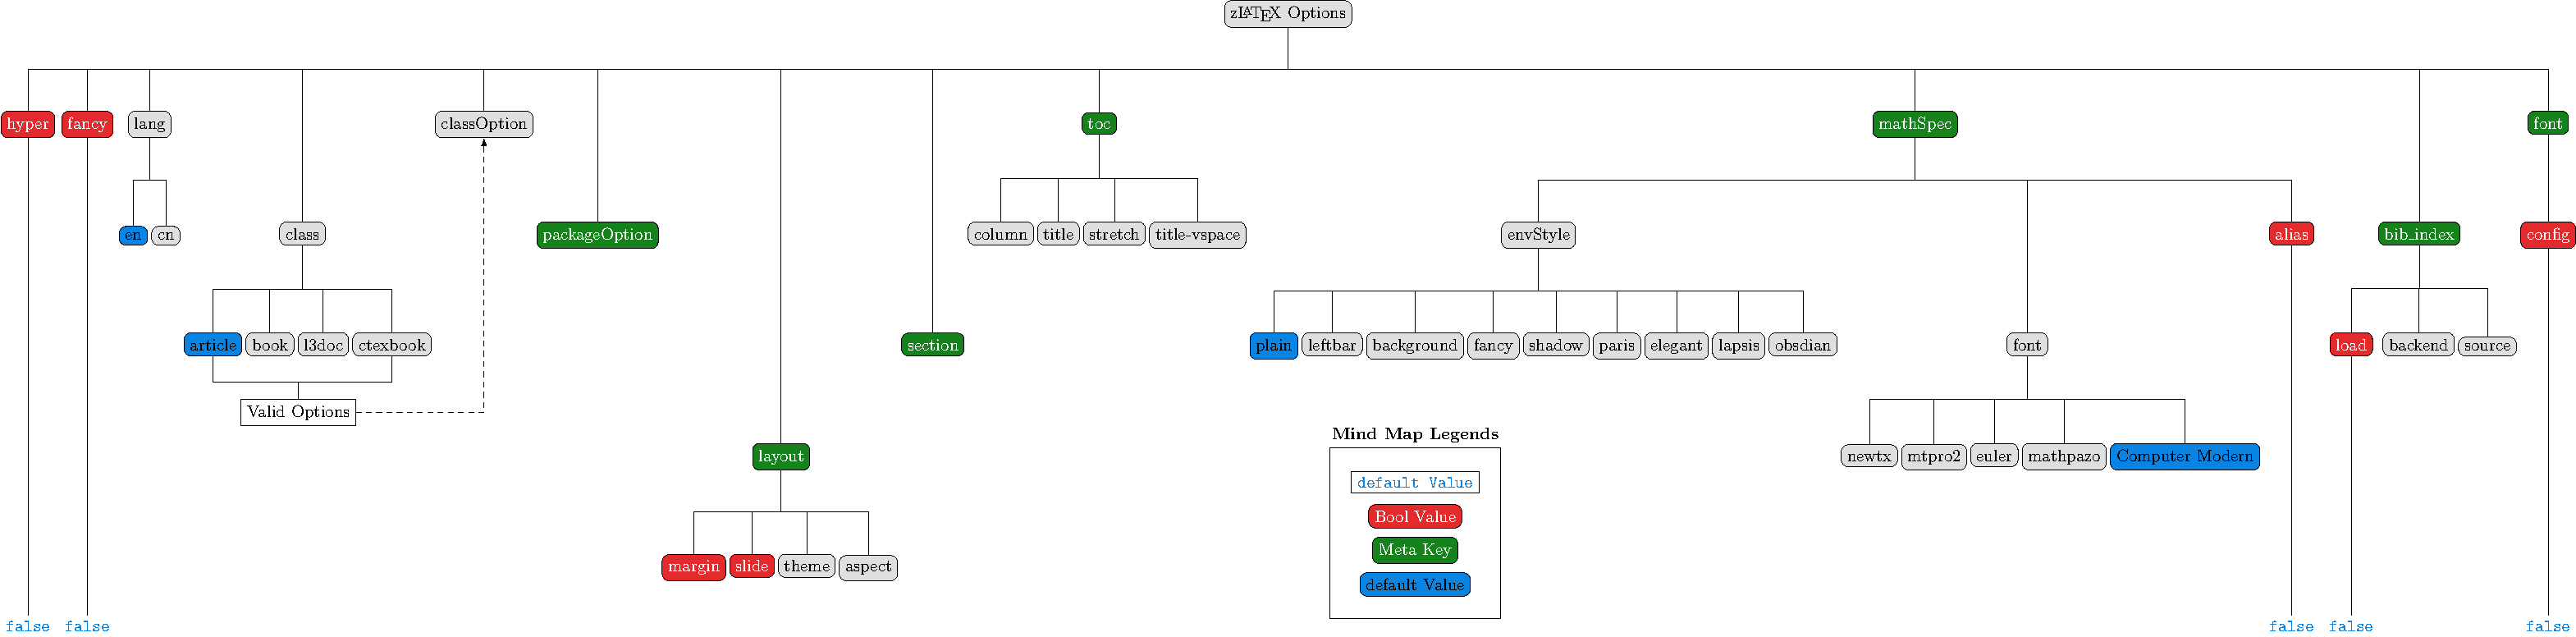
\includegraphics[width=1\linewidth]{./zlatex_options.pdf}
    \caption{zlatex options setup}
    \label{fig:zlatex-options}
\end{figure}

从\cref{fig:zlatex-options}可以看出, z\LaTeX{} 的配置是比较复杂的,但是刚接触本文档类时,用户也不必担心,默认的选项配置下
已经能够得到一个效果比较好的文档了.下面详细说明各个键的指定方式和作用. 

\subsection{classOption}
这里的\zkey{classOption}表示你加载的对应文档类的合法 options. 比如 {article} 文档类,合法的一个设置为:\cmd{classOption={10pt, oneside, fleqn}}. 
如果你在加载文档类时指定的\zkey{class}为 {ctexbook},那么此时你可以在\zkey{classOption} 中填诸如:\cmd{zihao=5, 12pt, heading=false, linespread=1.3} 
等 {ctex} 手册中说明的合法选项. 若对于默认的 article, book 文档类不熟悉,%
可以参见:\href{https://texblog.org/2013/02/13/latex-documentclass-options-illustrated/}{latex-documentclass-options}.

\subsection{packageOption}
传递参数给对应的宏包, 命令格式为:
\begin{minted}{latex}
\documentclass[
  lang=cn,
  packageOption={fontspec=quiet}
]{zlatex}
\end{minted}

如果某个宏包选项只给出了名称,而没有指定对应的 option,那么 z\LaTeX{} 会抛出警告.

\subsection{section}
调整章节标题格式的接口, 同样的, 此接口还没有开发完成.

\subsection{fancy}
这一选项为 bool 值, 目前仅 \cmd{\chapter} 命令和 \zkey{envStyle} 对此做了适配,后续可能会在此选项下开发更多的功能. 
\Footnote{值得一提的是: 当你的文档从 fancy 模式切换为普通模式后,可能会在编译过程中报错,这是正常的,直接忽略即可.}每个 chapter 对应的主题色
由 \cmd{zchapColor} 控制, 所以用户可以重定义此命令来改变章节的颜色主题.

fancy 章节中定义了一些列的元素, 它们均有一个默认的定义, 但是你可以引用下面的命令进行重定义:
\begin{itemize}
  \item \cmd{\zsubtitle{<content>}}: 章节的副标题
  \item \cmd{\zchapterSaying[<author>]{<saying>}}: 定义格言以及作者
  \item \cmd{\zchapterLContent{<content>}}: 章节左侧的内容, 不允许含有\texttt{\textbackslash par}等命令
  \item \cmd{\zchapterRContent{<content>}}: 章节右侧的内容, 不允许含有\texttt{\textbackslash par}等命令
\end{itemize}

一个使用样例:
\begin{minted}{latex}
\zsubtitle{Basic introduction to Chinese Culture}
\zchapterSaying[Xu Xiake]{The world is big, and I want to see it.}
\zchapterLContent{Xu Xiake(1587-1641) is a famous Chinese geographer and traveler.}
\zchapterRContent{He is known for his extensive travels throughout China.}
\end{minted}

后页展示了部分使用样例:
% \begin{figure}[!htb]
%   \centering
%   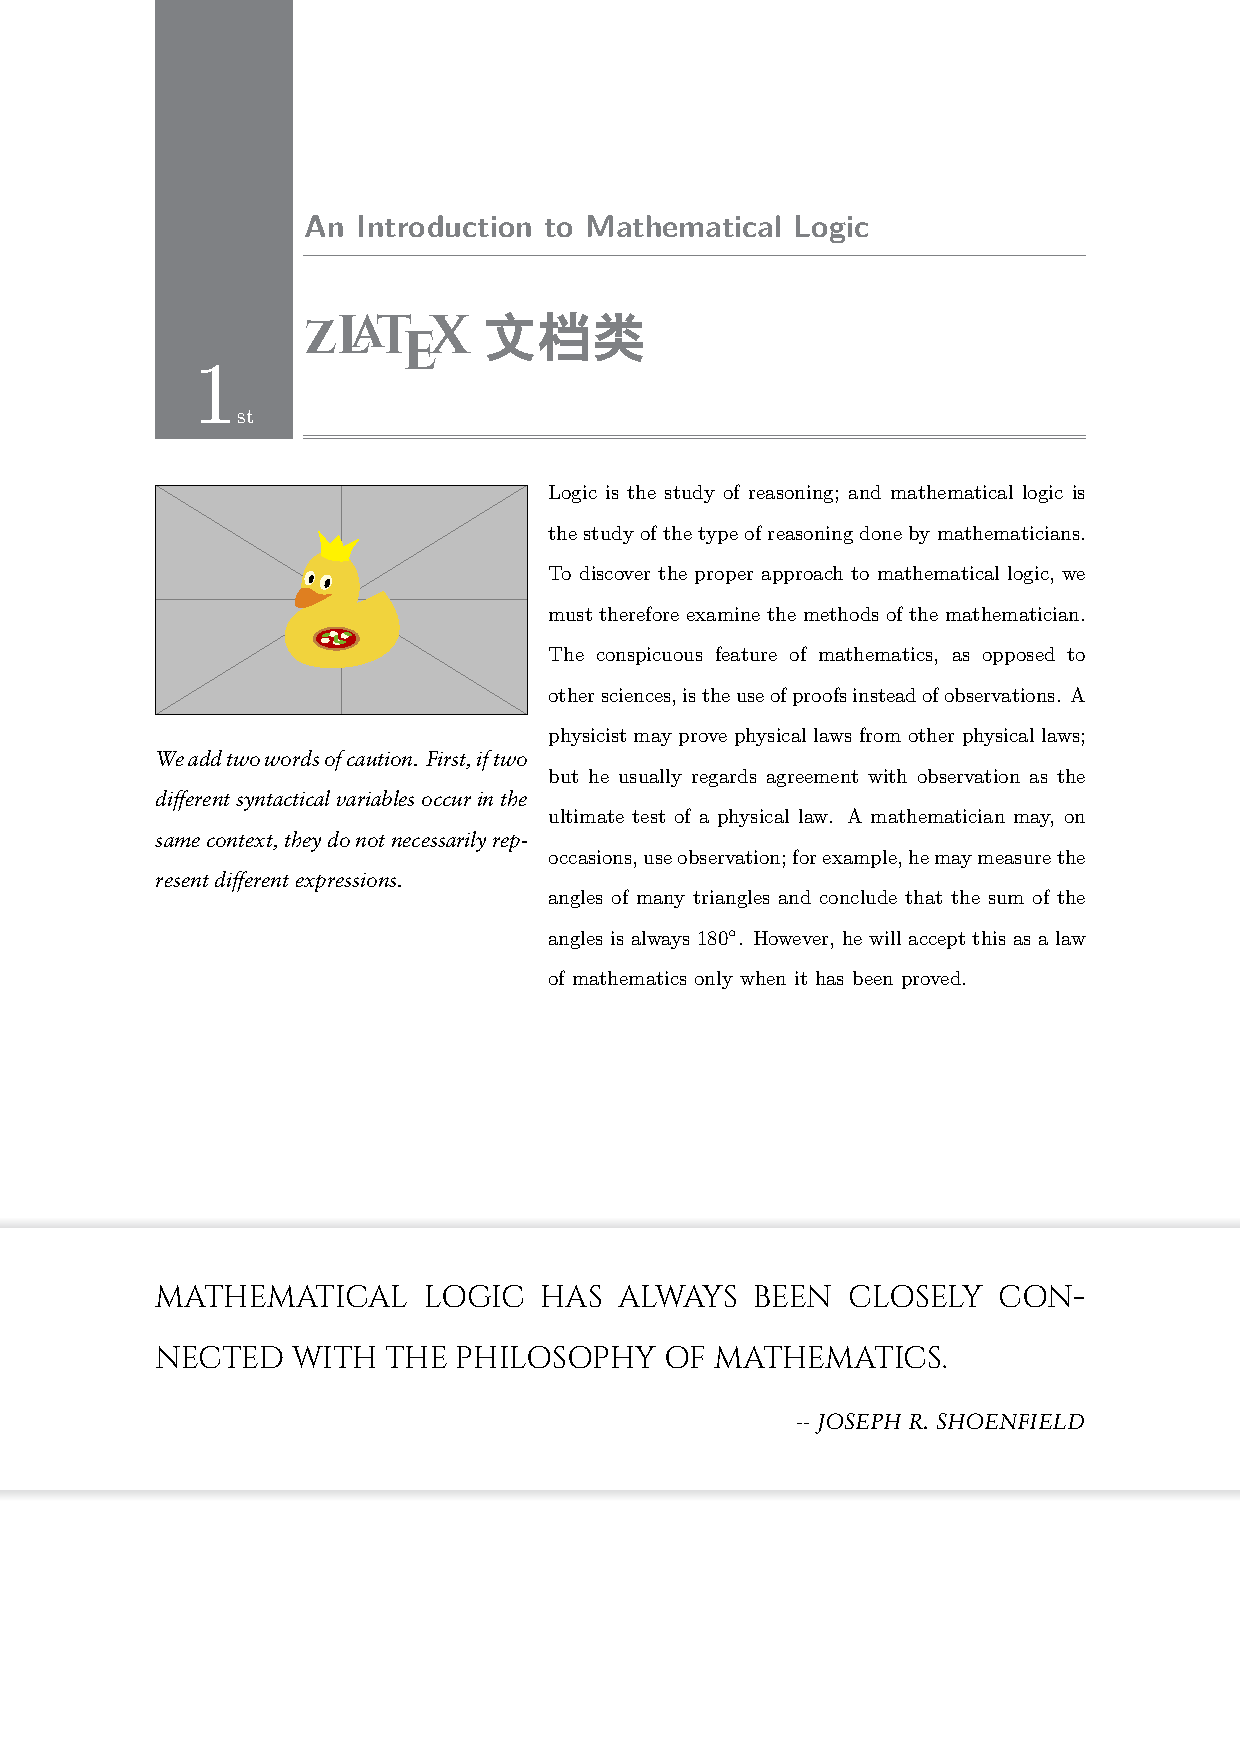
\includegraphics[width=.45\linewidth]{./fancy_chapter_1.pdf}
%   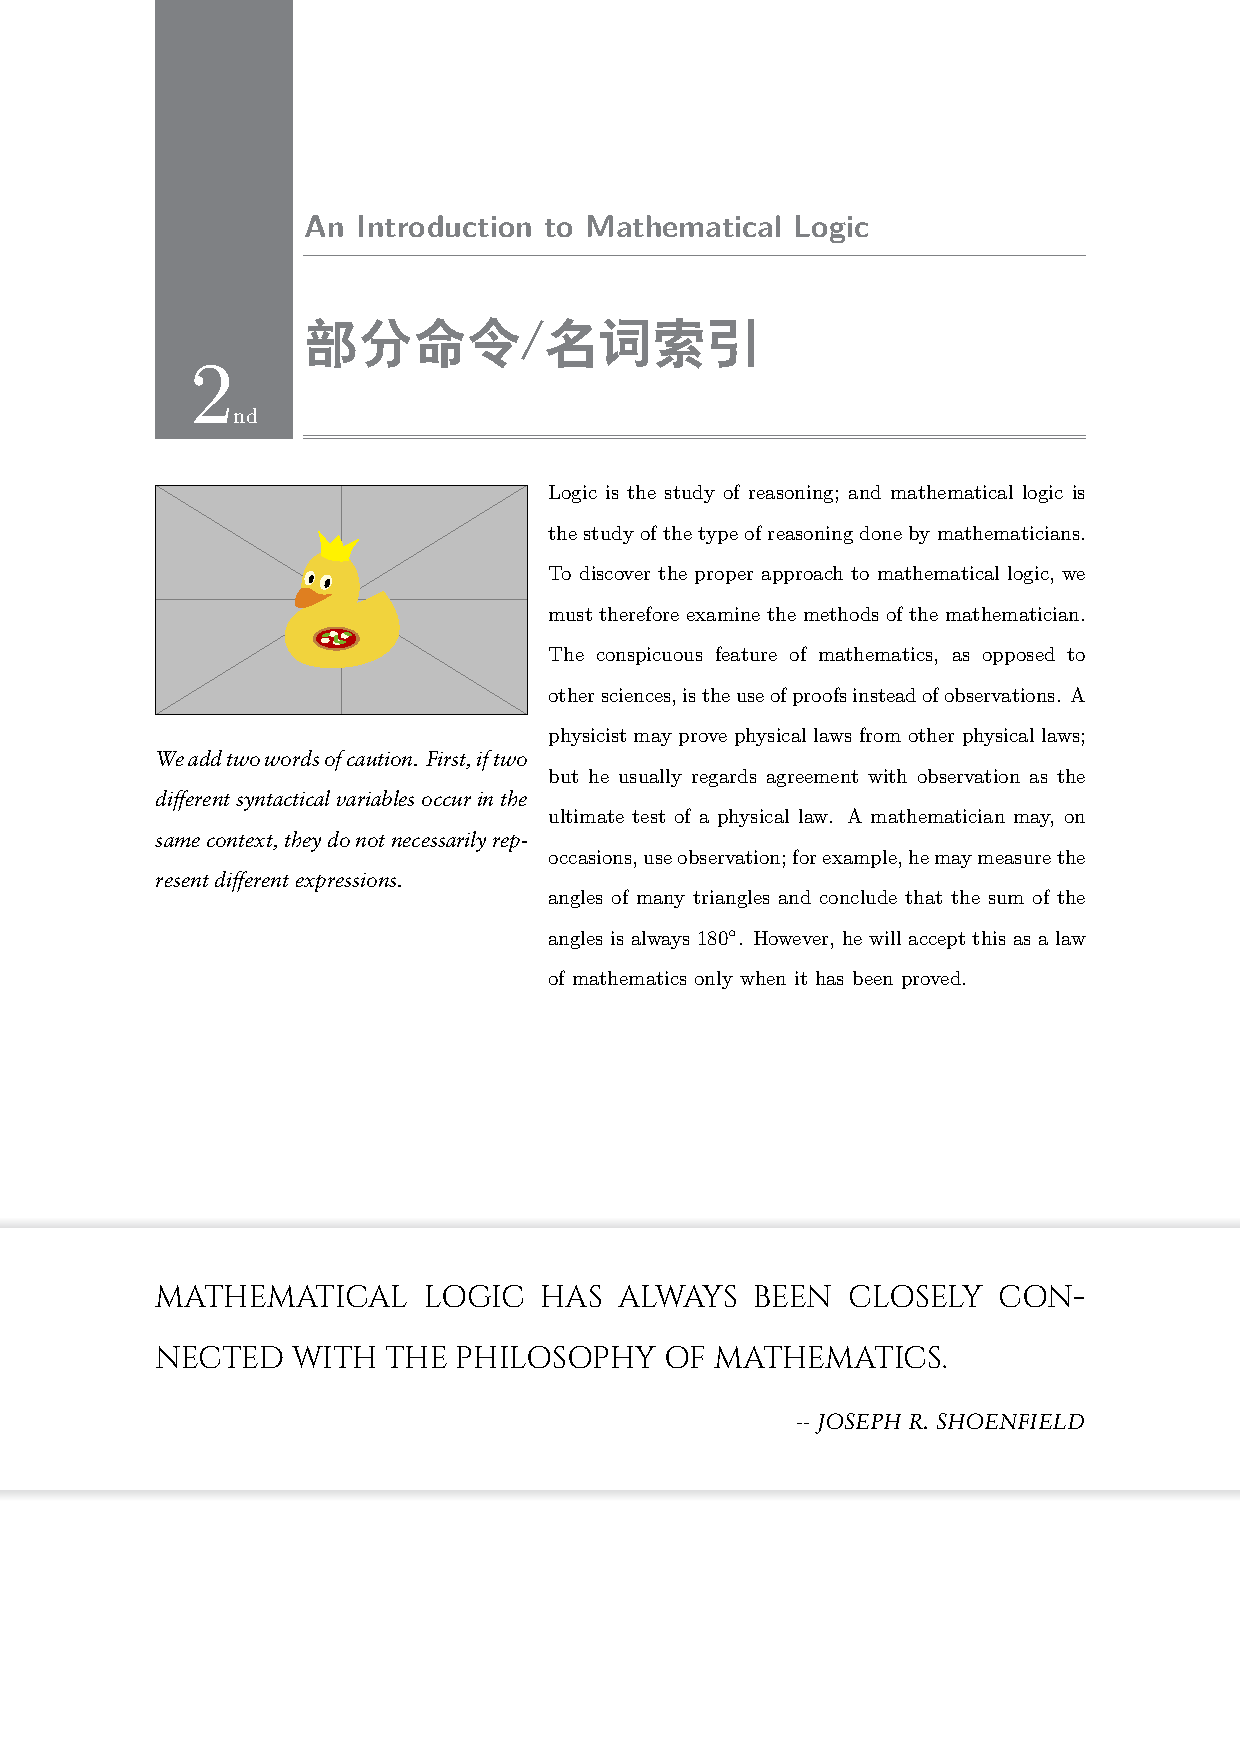
\includegraphics[width=.45\linewidth]{./fancy_chapter_2.pdf}
  
%   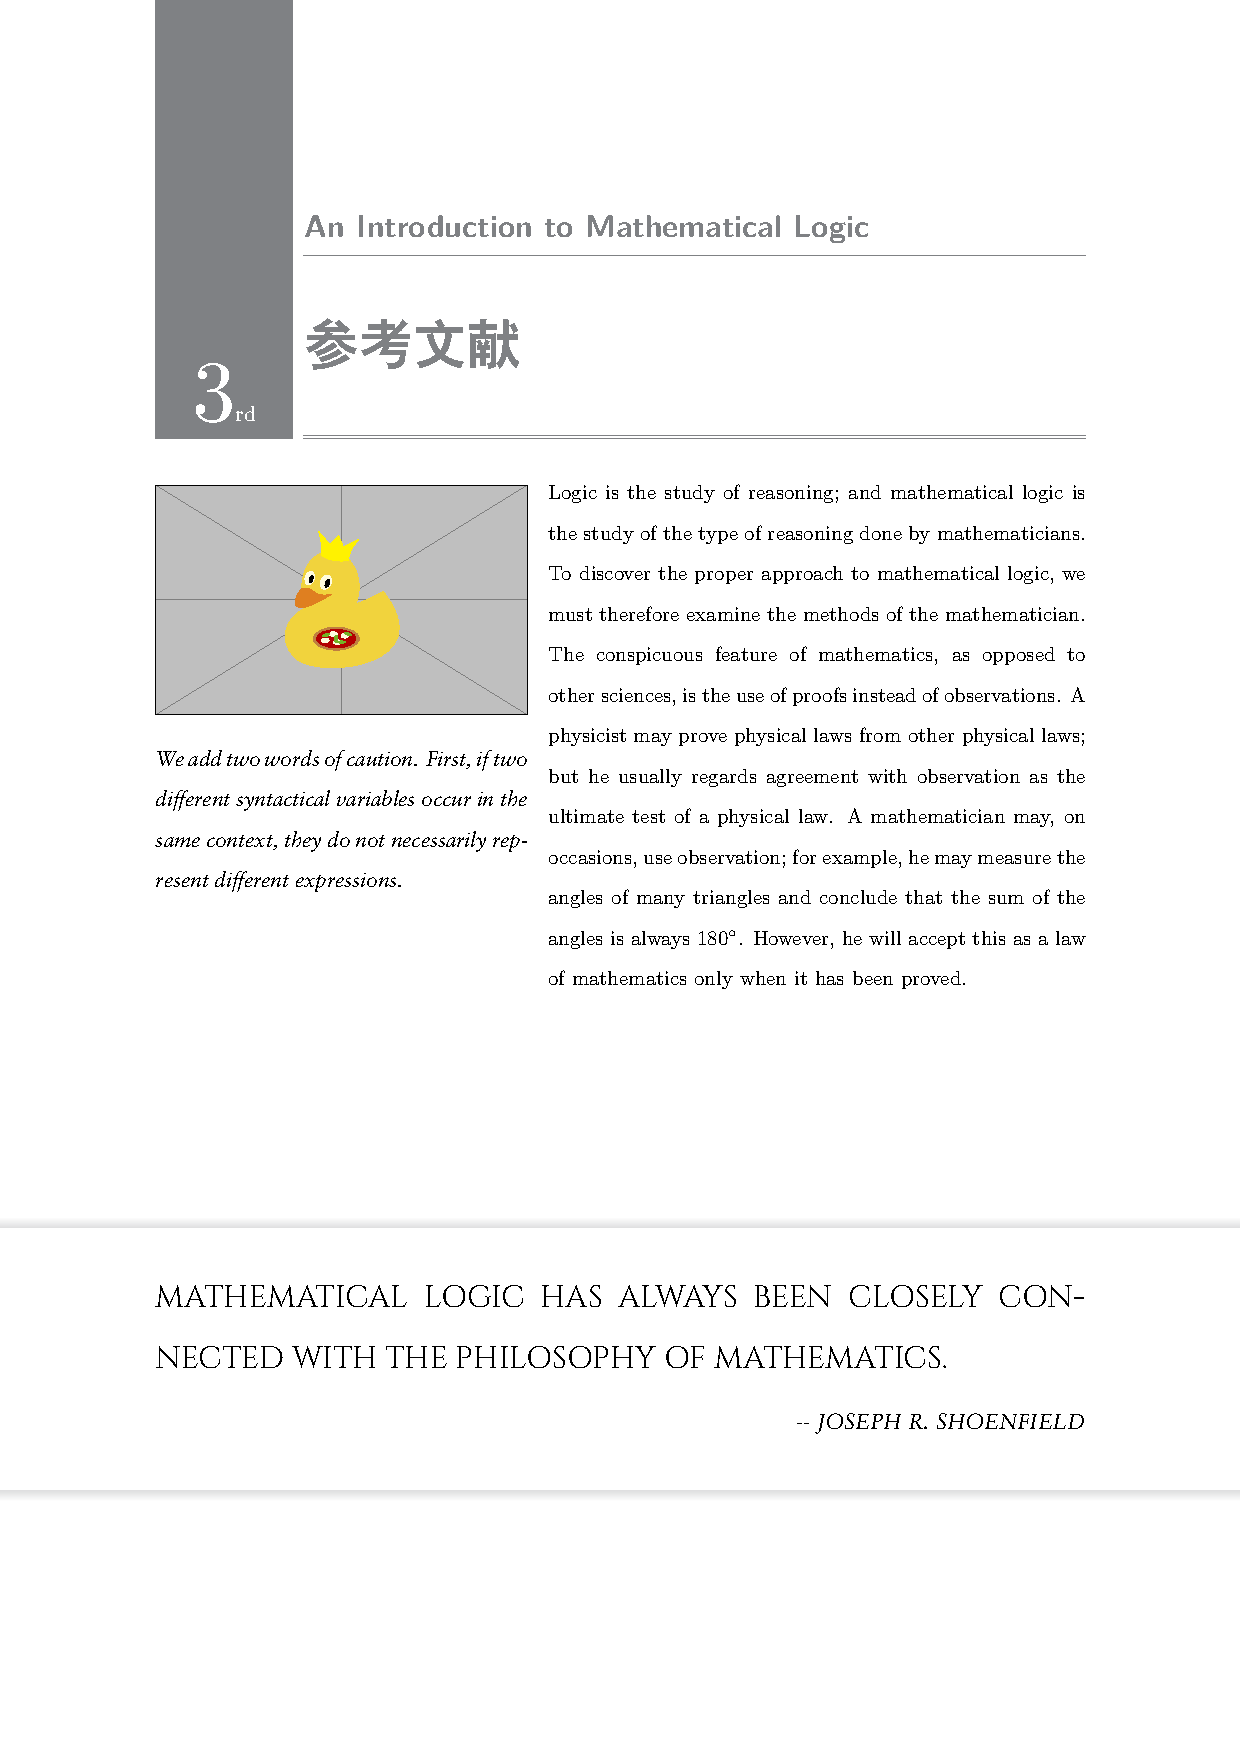
\includegraphics[width=.45\linewidth]{./fancy_chapter_3.pdf}
%   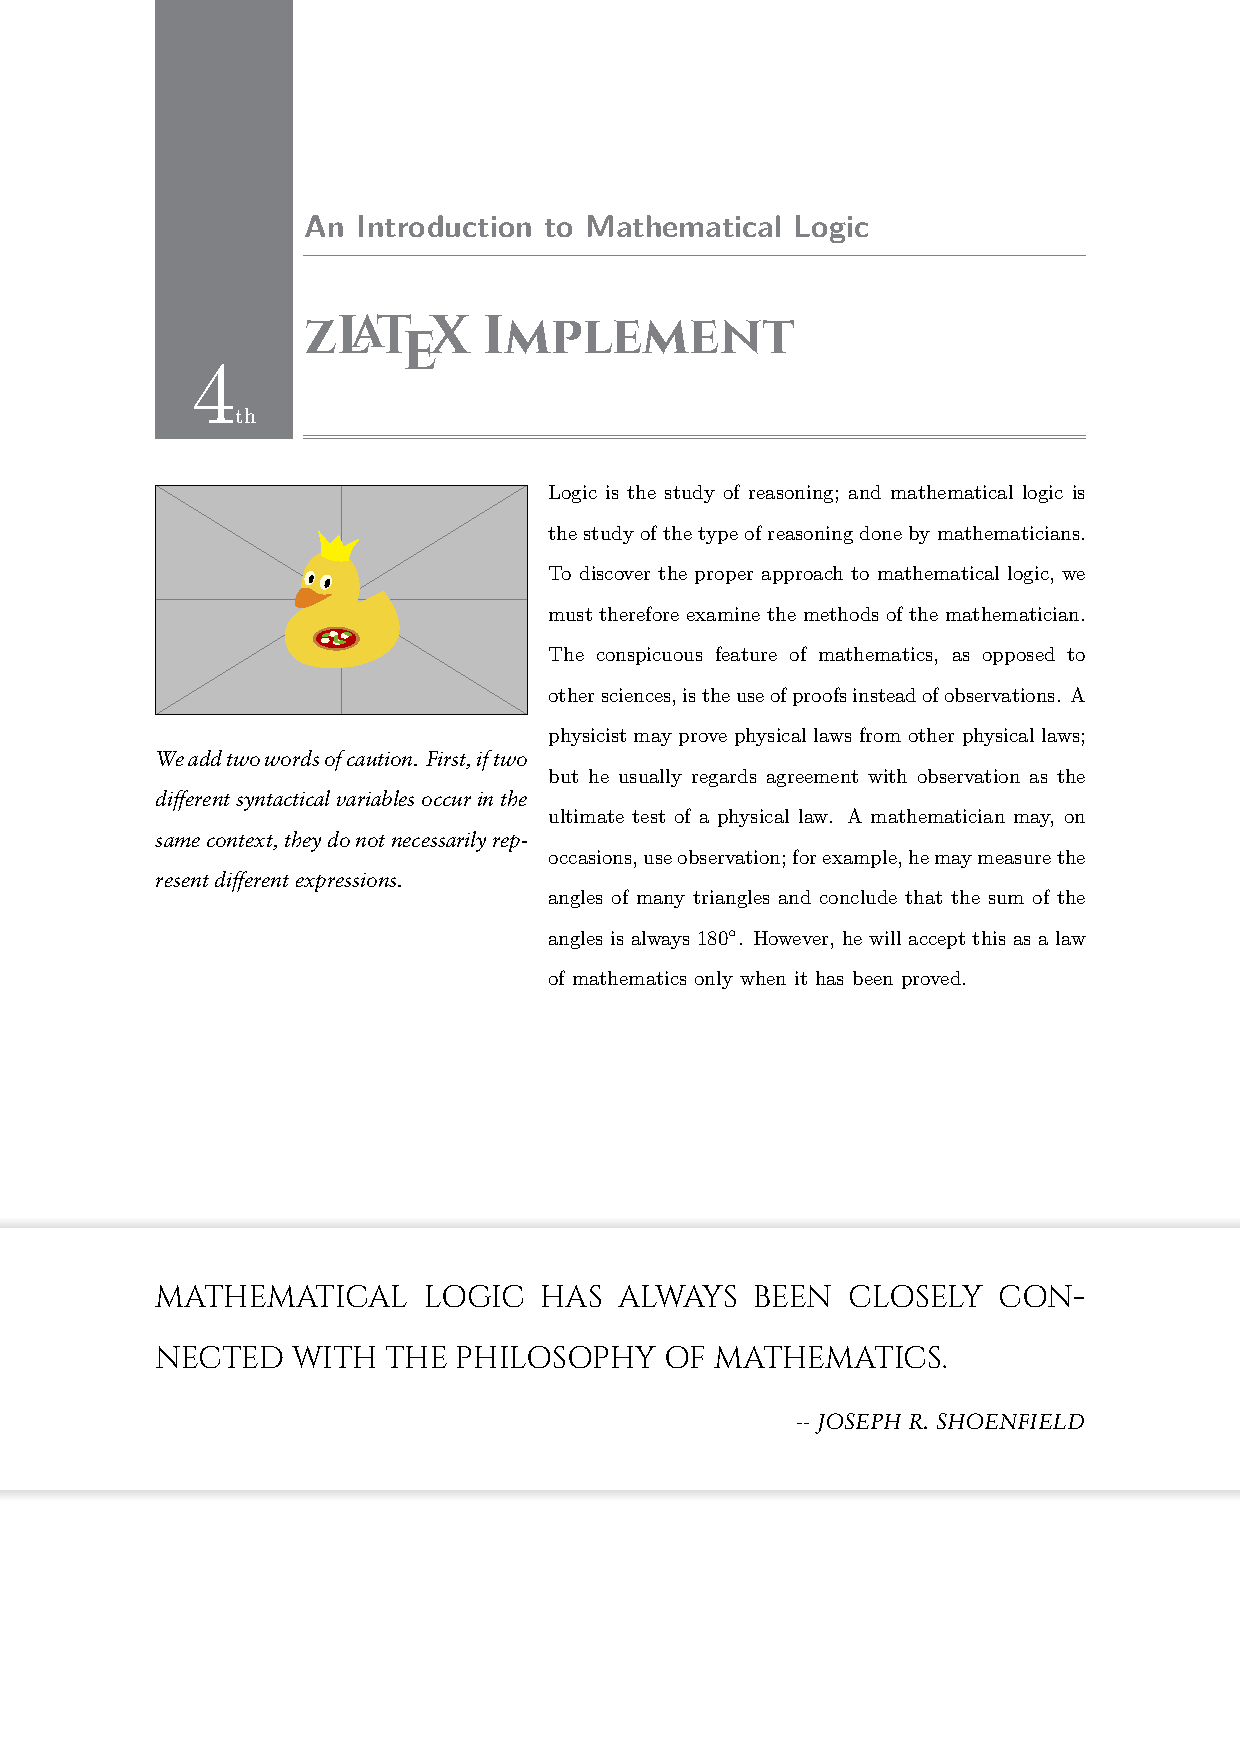
\includegraphics[width=.45\linewidth]{./fancy_chapter_4.pdf}
%   \caption{fancy chapter Examples}
%   \label{fig:fancy-chapter-examples}
% \end{figure}

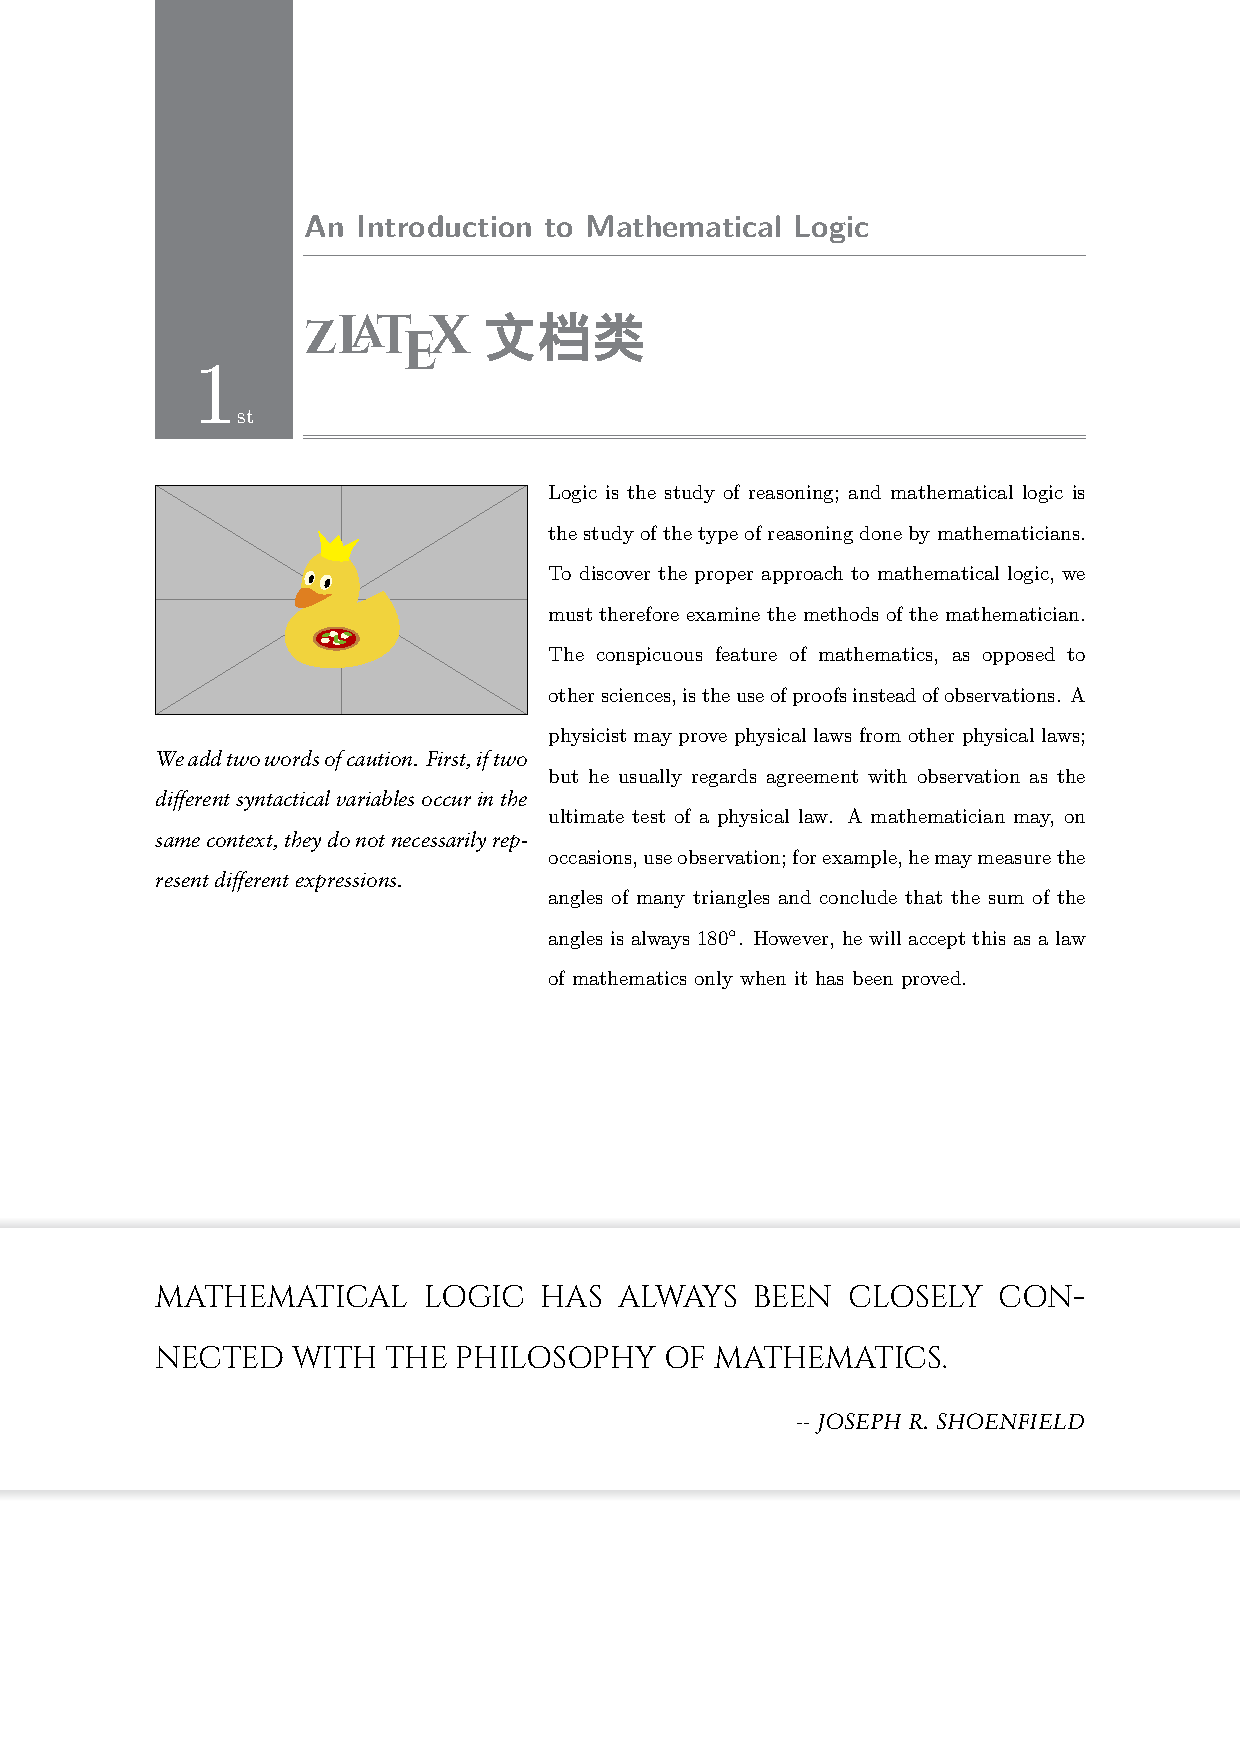
\includepdf[frame, nup=2x1, pages=-, delta=8 8]{fancy_chapter_example.pdf}

\subsection{lang}
键\zkey{lang}的合法值为 {en, cn}; 第二个关于文档语言的指定是比较容易理解的,但是还是得说明对应的一些注意事项.\cmd{lang=cn}或者\cmd{class=ctexbook}时
仅支持为\hologo{XeLaTeX}编译;在指定\cmd{lang=en}时, \hologo{pdfLaTeX}, \hologo{XeLaTeX} 二者都是可以接受的,但是建议使用 \hologo{pdfLaTeX}. 因为在指定\cmd{lang=en}时部分的西文宏包
可能会有冲突的危险.当指定\cmd{lang=en}, 并且采用 \hologo{pdfLaTeX} 进行编译时,z\LaTeX{}会引入宏包 {inputenc}, 然而此宏包对 \hologo{XeLaTeX} 是
没有适配的.

\subsection{toc}
键\zkey{toc}\index{\cmd{toc}}的合法值为\cmd{column, title, title-vspace}, 这一选项主要用于文档的目录格式设置,可以设置目录页对应的标题,目录的栏数.
\zkey{column}选项用于指定目录栏数, 默认为1. \zkey{title} 用于指定目录名,默认为 ``Contents'' 或 ``目录''. \zkey{title-vspace} is self-explanatory.
如果要自定义更加复杂的目录格式,下述即为一个样例:

\begin{minted}{latex}
% use class option
\documentclass[
  toc={title=CONTENTS, column=2},
]{zlatex}

% use \zlatexSetup command
\zlatexSetup{
  toc={
    column = 2,
    title=\hfill\large\normalfont CONTENTS {\sffamily\small NEW}\hfill
  }
}
\end{minted}

\begin{remark}
由于整个 title 的内容均位于 \cmd{\section*{<title>}} 内, 所以请不要输入类似 \cmd{\par} 等命令. 同时,如果在加载文档类时指定目录名,
那么其中不能包含任何的控制序列, 如果需要包含任何的控制序列,请使用命令 \cmd{\zlatexSetup} 进行设置. 
\end{remark}

\subsection{bib\_index}
\zkey{bib\_index} 用于控制 indextools 和 biblatex 等宏包的加载,默认不加载这两个宏包. 针对参考 biblatex 宏包, 本模板的默认参考文献
编译后端为 {biber},可以在导言区通过\cmd{backend=bibtex}来更改默认后端为\cmd{bibtex}.这说明,在默认配置下,你编译文档时应在命令行
使用 {biber} 命令, 而非 {bibtex} 命令. 同样的,可以通过\zkey{bib}的子键\zkey{source}来指定参考文献对应的文件名,默认文件名为: {ref.bib}. 

针对于索引格式定制所需的 .ist 文件, 目前还需用户在命令行编译时手动指定.

\subsection{layout}\label{sec:slide-mode}
\mstyle{基本介绍}
z\LaTeX{} 默认页面布局如:\cref{fig:zlatex-default-layout}
\begin{figure}[!htb]
  \centering
  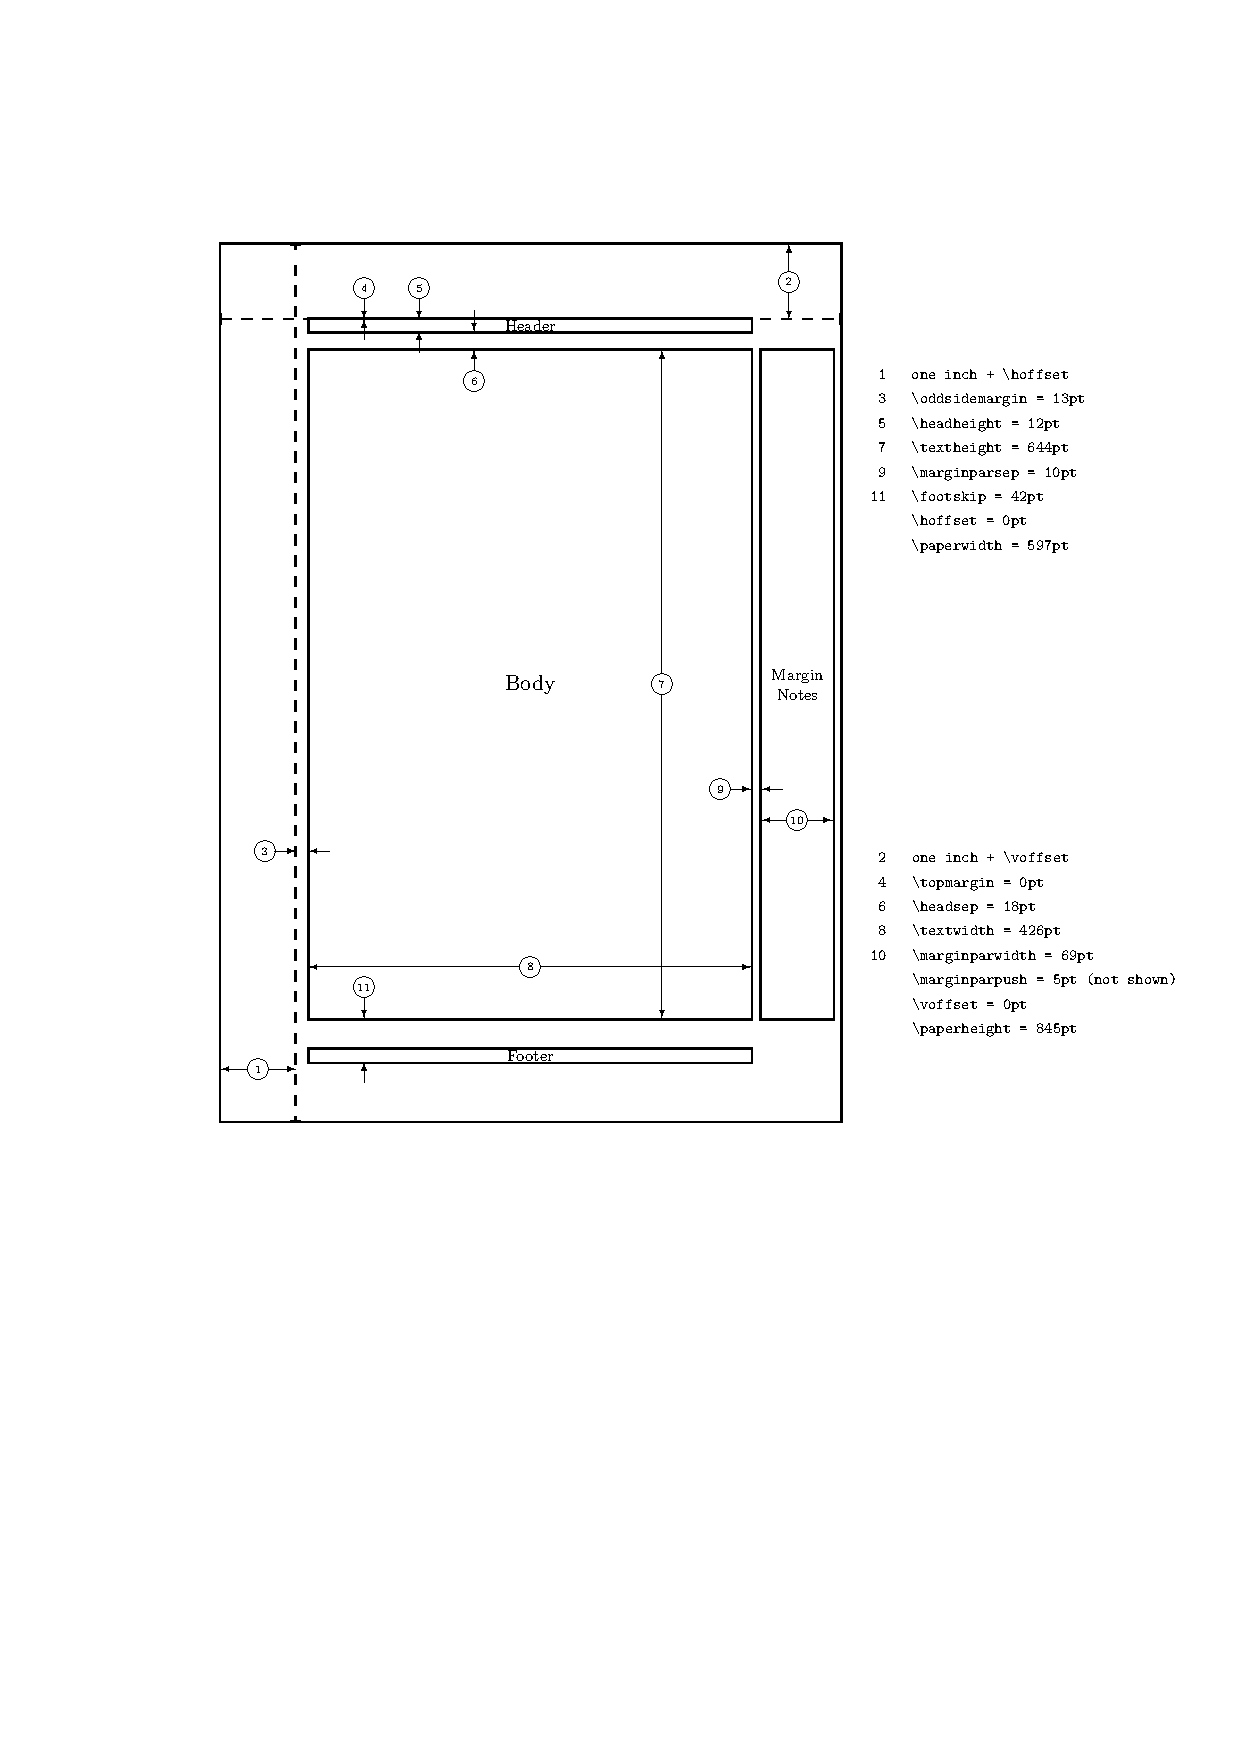
\includegraphics[width=.9\linewidth]{./zlatex_layout_default.pdf}
  \caption{z\LaTeX{} default page layout}
  \label{fig:zlatex-default-layout}
\end{figure}

\zkey{layout} 键可用于指定整个文档布局:版心,页边距,边注间距等,也可以指定文档最终的呈现方式:普通的文档,还是展示所用的slide.
目前模板提供子键\zkey{margin, slide}用于设置对应布局. 此键合法值为bool值, 指定方式如下:
\begin{minted}{latex}
% {margin} <=> {margin=true}
\documentclass[
  layout={margin, slide}
]{zlatex}
\end{minted}

默认情况下\zkey{margin}的值为\cmd{false}. 如果使用了上述键值指定,那么此时的文档就会产生一个边注. 一般情况下,如果不是撰写相应的书籍,
使用者是不需要加载这个选项的. \textbf{需要注意}:\cmd{margin=false} 只有在\cmd{oneside} 时才有效,否则会抛出警告. 如果原文档中含有\cmd{\marginpar}
命令,那么在指定\cmd{margin=false}后,对应的\cmd{\marginpar}环境,会被替换为\cmd{framed}宏包提供的\cmd{leftbar}环境.

\begin{remark}
默认情况下 \cmd{twoside} 选项对应的 margin 和 \cmd{margin} 选项对于的 margin 宽度是不同的,后者比前者宽一些.
\end{remark}

\subsection{slide Mode}\index{slide mode}
\mstyle{ascpect ratio}
如果你需将最终的文档编译为演示文档, 除了必须加载\zkey{slide}选项外,你还可以指定幻灯片比例, 使用\zkey{aspect}子键进行设置,
默认的比例为\cmd{16:9},默认的长度单位为厘米(cm). 如果你想要设置幻灯片的比例为12:9,那么导言区按照如下设置即可:
\begin{minted}{latex}
\documentclass[
  layout={slide, aspect=12|9},
]{zlatex}
\end{minted}

也就是使用符号``|''进行两个维度上距离的分割. 


\mstyle{slide theme}
slide 模式下,用户可以自由切换主题颜色. 出于加载速度考虑,主题的指定应在导言区声明, 即指定 \zkey{layout/theme}. 
zlatex 内置了四套主题色彩,内置主题命令方式为: <beamer-theme-name>-<beamer-themecolor-name>. 目前 zlatex 只复刻了 
beamer 下的 {AnnArbor} 主题,但是内置了4中色彩主题:
\begin{itemize}
  \item AnnArborDefault
  \item AnnArborBeaver
  \item AnnArborAlbatross
  \item AnnArborSeahorse
\end{itemize}

在导言区指定对应的主题后,如果用户希望在加载某一个主题的时同时覆盖一部分主题的原定义,可以使用命令:
\begin{minted}{latex}
\zslideThemeUse[UL={text=UL-TEXT}]{<theme-name>}
\end{minted}

\mstyle{自定义主题}
目前 slide 模式下还不支持自定义主题,因为这部分涉及到的内容比价繁杂,还没有考虑好如果实现. 但是用户可以通过重定义对应的颜色来实现自定义主题,
请参见后文的示例.

\mstyle{自定义主题}
slide 模式下的主题颜色\index{slide theme}目前基本均由三名称控制,用户如果想要修改 slide 的主题色,请重定义它们。以下展示默认主题色对应的
三个颜色定义:

\definecolor{Ann-default-I}{HTML}{0000a3}
\definecolor{Ann-default-II}{HTML}{ffc20c}
\definecolor{Ann-default-III}{HTML}{ffcb03}

\begin{table}[H]
\begin{tblr}{
    colspec={X[1, c]X[1, c]X[1, c]},
    rowspec={Q[m]Q[m]}
  }
  Ann-default-I: \block{Ann-default-I} &
  Ann-default-II: \block{Ann-default-II} &
  Ann-default-III: \block{Ann-default-III}
\end{tblr}
\end{table}

用户不仅可以自定义主题,还可以自定义对应的 metadata. 目前 slide 模式下提供的命令\cmd{\zslideThemeCreate}\index{\cmd{zslideThemeCreate}} 
可以设置这部分的 metadata,即 slide 的基本信息展示. 命令的基本使用格式为:

\begin{minted}{latex}
\zslideThemeCreate{<theme-name>}{<theme-spefication>}
\end{minted}

一个简单的自定义主题并且应用此主题的示例如下:
\begin{minted}{latex}
% create theme
\zslideThemeCreate{test}{
  UL={text=UL-TEXT},
  UR={text=UR-TEXT},
  sec={bg=black, fg=white, prefix=\ding{100}}
  % toc setting
  toc={
    leftmargin = {section=10em, subsection=15em},
  }
}

% use this theme
\zslideThemeUse{test}
\end{minted}

每一个 \texttt{<meta key>} 的细节请自定指定. 目前 \zkey{UL, UR} 对应的 content 默认位于右侧与左侧. 如果 
用户需要定义比较复杂的页面样式,请自己定义对应的条件判断函数. 本模式下,定义了命令 \cmd{\pageref{zslide-last-page}}
\index{zslide-last-page}用于索引演示文稿的总页面数目. 

用户还可以指定 slide 模式下的目录格式, frame 的章节栏格式,设置的方法如上,只需指定对应的键值即可.

为了给刚开始使用的用户一个完整的设置样例,请看下面的代码, 此即为内置主题的定义:
\begin{minted}{latex}
\zslideThemeCreate {AnnArborDefault}{
  doc = {
    bg-color = white,
    text-color = black,
    text-style = \sfdefault
  },
  UL = {
    bg   = Ann-default-I,
    fg   = Ann-default-II,
    text = {\ifnum\arabic{section}=0\else Section\ \thesection\fi}
  },
  UR = {
    bg   = Ann-default-II,
    fg   = Ann-default-I,
    text = {\ifnum\arabic{subsection}=0\else Subsection\ \thesubsection\fi}
  },
  BL = {
    bg   = Ann-default-I,
    fg   = Ann-default-III,
    text = \zslideAuthor
  },
  BC = {
    bg   = Ann-default-III,
    fg   = Ann-default-I,
    text = \zslideTitle
  },
  BR = {
    bg   = Ann-default-II,
    fg   = Ann-default-I,
    text = \zslideDate\quad \thepage/\pageref{zslide-last-page}
  },
  sec = {
    fg   = Ann-default-I,
    bg   = Ann-default-III,
    prefix = {},
    suffix = {}
  }
}
\end{minted}


\mstyle{简单示例}
后页内容即为一个简单的 slide 模式示例:
% \cref{fig:slide-example} 为一默认 slide 模式样例:
% \begin{figure}[!htb]
%   \centering
%   
\includegraphics[width=.85\linewidth]{./doc2slide_1.pdf}
%   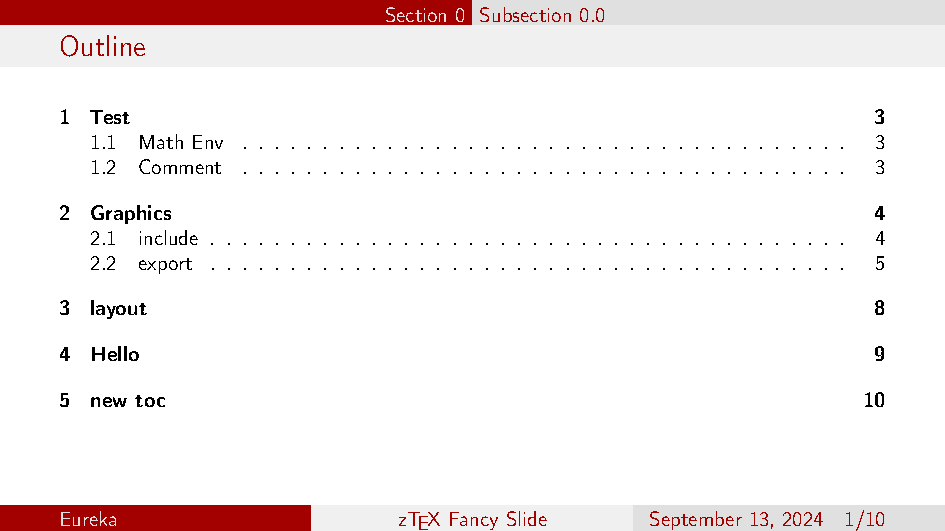
\includegraphics[width=.45\linewidth]{./doc2slide_2.pdf}
%   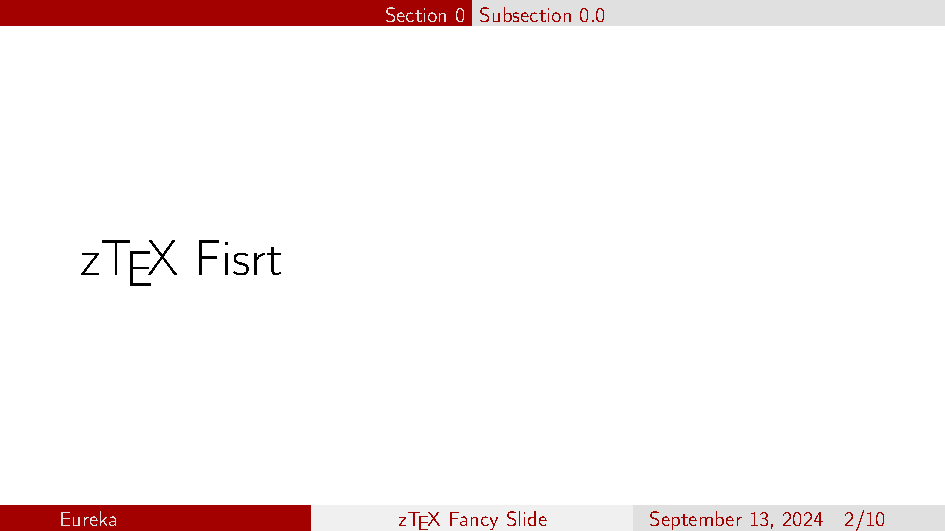
\includegraphics[width=.45\linewidth]{./doc2slide_3.pdf}
%   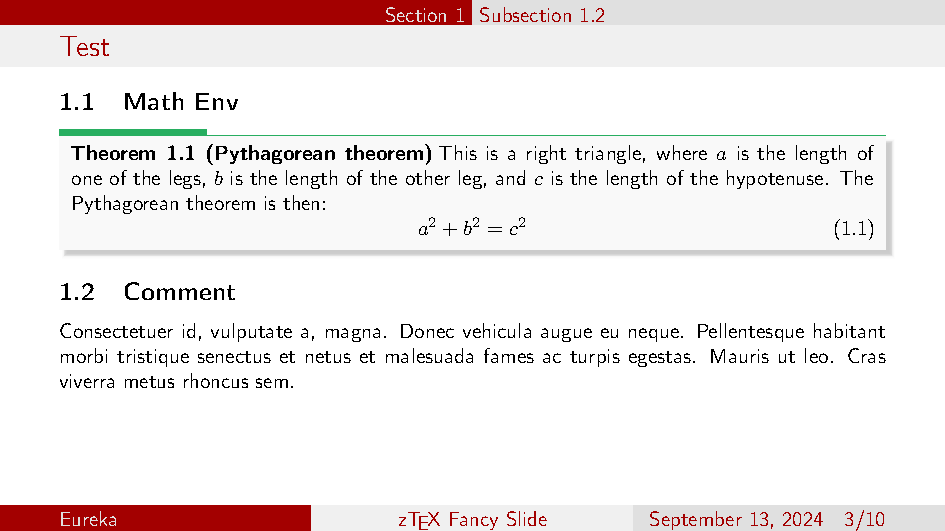
\includegraphics[width=.45\linewidth]{./doc2slide_4.pdf}
%   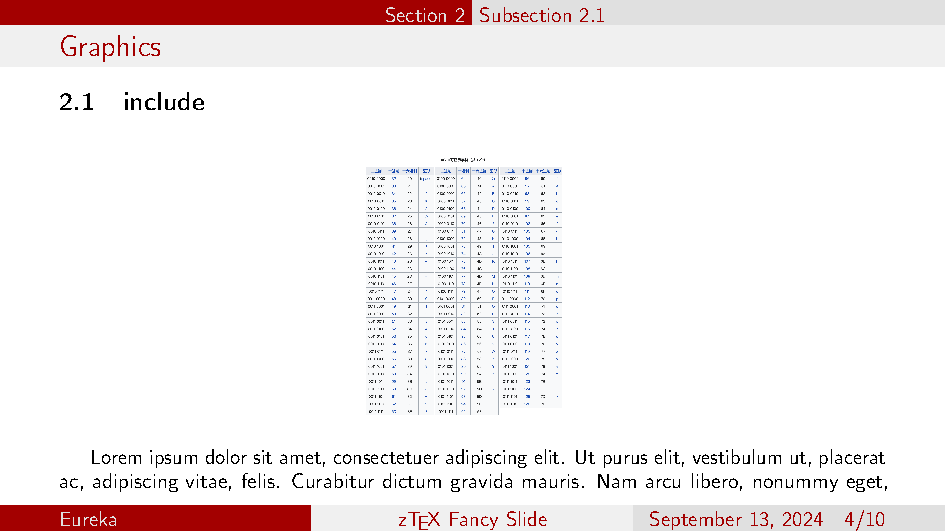
\includegraphics[width=.45\linewidth]{./doc2slide_5.pdf}
%   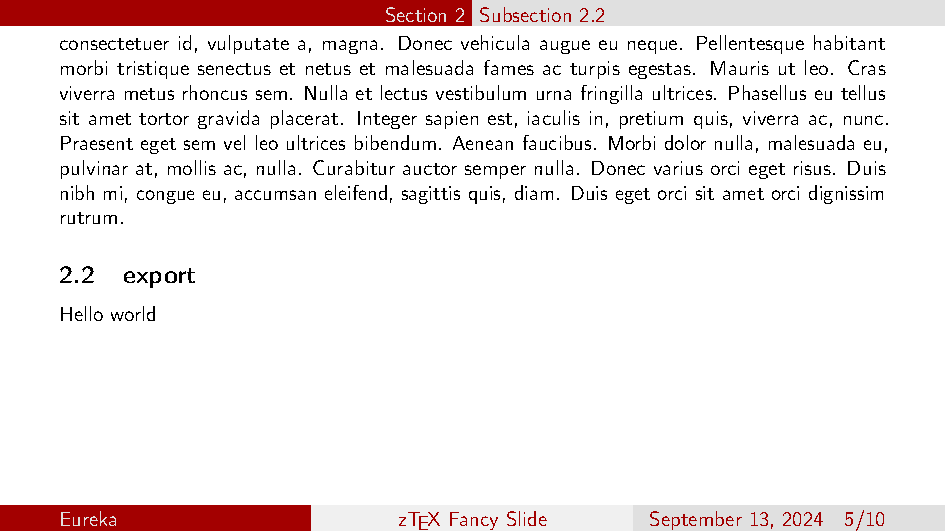
\includegraphics[width=.45\linewidth]{./doc2slide_6.pdf}
%   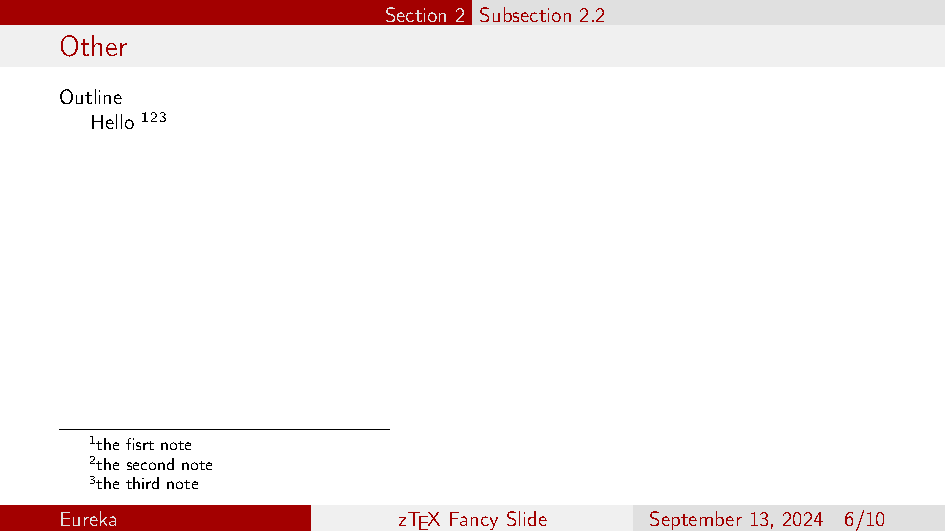
\includegraphics[width=.45\linewidth]{./doc2slide_7.pdf}
%   \caption{Slide 样例}
%   \label{fig:slide-example}
% \end{figure}

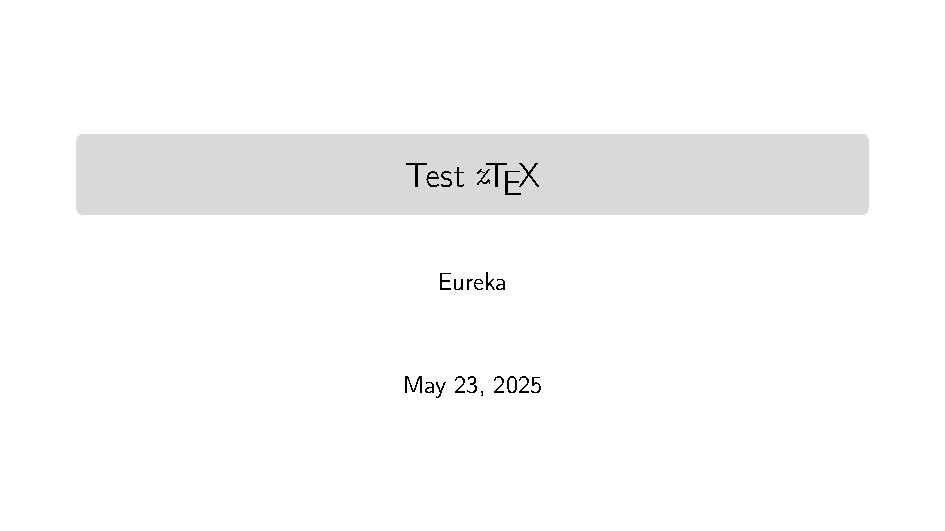
\includepdf[frame, nup=3x5, pages=-, delta=8 8]{zslide_example.pdf}


\mstyle{remark}
目前 slide 模式还处于一个不太成熟的阶段,请谨慎使用. 正式场合下还请使用默认的 beamer 文档类.

由于本模板可以切换单双面布局,所以为了保证 titlepage 中文字的正确居中,本文档类对原始命令:\cmd{\maketitle} 进行了重定义,
原始的定义保存在 \cmd{\orimaketitle} 中. 为定义本文档类的 \cmd{\maketitle} 命令格式,部分页面布局下,标题可能无法居中,
所以在必要的情况下,请自定义格式. 在 slide mode 下,本文档类提供了 \cmd{\zslideTitle,\zslideAuthor,\zslideDate} 三个
可以多次使用的命令\Footnote{众所周知,\texttt{\textbackslash maketitle} 会清除 \texttt{\textbackslash @title, \textbackslash @author, \textbackslash @date} 的定义}.

\mstyle{Hacker Note}
为了从 book 或 article 过渡到 slide,z\LaTeX{} 在背后做了相当部分的工作,包括但不限于:
\begin{itemize}
  \item 页面 background 设置 
  \item slide 的 metadata 设置
  \item \cmd{\chapter,\section}等命令的重定义
  \item 页面布局重定义
\end{itemize}

由于 slide 的 metadata 主要依靠 fancyhdr 宏包提供的接口, 所以 metadata 的位置可能会随着页面布局,
字体大小的改变产生一些微小的一些变化. slide 布局下,所应用的钩子如下:
\begin{minted}{latex}
% status bar and metadata-item
\bool_new:N \g_new_sec_bool
\AddToHook{cmd/chapter/before}{\newpage}
\AddToHook{cmd/section/before}{\newpage}
\AddToHook{shipout/firstpage}{\setcounter{page}{0}}
\AddToHook{shipout/lastpage}{\label{zslide-last-page}}
\AddToHook{shipout/after}{\bool_gset_false:N \g_new_sec_bool}
\AddToHook{cmd/tableofcontents/before}{\renewcommand{\contentsname}{Outline}}
\AddToHook{shipout/background}{
  \put(0, -\paperheight){\textcolor
      {\tl_use:N \l__zlatex_slide_doc_bgcolor_tl}
      {\rule{1\paperwidth}{1\paperheight}}}
}
\AddToHook{shipout/background}{
  \_zslide_status_bar:nnnn {UL}{(0,              -.9em)}{.5}{1.25em}
  \_zslide_status_bar:nnnn {UR}{(.5\paperwidth,  -.9em)}{.5}{1.25em}
  \_zslide_status_bar:nnnn {BL}{(0,              -\paperheight)}{.33}{.9em}
  \_zslide_status_bar:nnnn {BC}{(.33\paperwidth, -\paperheight)}{.34}{.9em}
  \_zslide_status_bar:nnnn {BR}{(.67\paperwidth, -\paperheight)}{.33}{.9em}
  \bool_if:NT \g_new_sec_bool {
  \_zslide_status_bar:nnnn {sec}{(0, -2.7em)}{1}{1.8em}}
}
\AddToHook{shipout/foreground}{
  \_zslide_status_info:nnnn {head}{ 0 }{.5 }{ \hfill\_slide_metadate:n {UL}\  }
  \_zslide_status_info:nnnn {head}{.5 }{.5 }{ \ \_slide_metadate:n {UR}\hfill }
  \_zslide_status_info:nnnn {foot}{ 0 }{.33}{ \hfill\_slide_metadate:n {BL}\hfill }
  \_zslide_status_info:nnnn {foot}{.33}{.34}{ \hfill\_slide_metadate:n {BC}\hfill }
  \_zslide_status_info:nnnn {foot}{.67}{.33}{ \hfill\_slide_metadate:n {BR}\quad  }
  \exp_args:Ne \hyper@anchor{zslide@\FirstMark{zslide-left}.\int_use:N \g__zlatex_slide_framecnt_int}
}
\cs_new_protected:Npn \_zslide_status_bar:nnnn #1#2#3#4 {
  \ifnum\thepage=0\else
    \put#2 {\textcolor{\tl_use:c {l__zlatex_slide_#1_bg_tl}}{\rule{#3\paperwidth}{#4}}}
  \fi
}
\cs_new_protected:Npn \_zslide_status_info:nnnn #1#2#3#4 {
  \ifnum\thepage=0\else\str_case:nn {#1}{ 
    {head} {\put(#2\paperwidth, -.9em+2.5pt) {\hbox~ to~ #3\paperwidth {#4}}}
    {foot} {\put(#2\paperwidth, -\paperheight+2.5pt) {\hbox~ to~ #3\paperwidth {#4}}}
  }\fi
}
\end{minted}

所以,如果用户需要重定义这部分钩子的行为,请在一定程度上参考上述命令的实现.

\subsection{font}\index{z\LaTeX{} Font Setup}
目前此接口还处于早期开发阶段,目前仅对 \cmd{\Cinzel} 这一字体族做了兼容, 用户如果在本地安装有字体 Cinzel, 
那么可以在导言区加载对应的选项, 如下:
\begin{minted}{latex}
\documentclass[
  ...
  font={config},
  ...
]{zlatex}
\end{minted}

加载此选项后,fontspec 会去寻找对应字体进行如下设置
\begin{minted}{latex}
\RequirePackage{fontspec}
\newfontfamily{\Cinzel}{CinzelRegular.ttf}[
  BoldFont=CinzelBold.ttf,
  ItalicFont=SabonItalic.ttf
]
\end{minted}

若本地并没有安装对应字体,用户可以忽略此选项. 需要注意的是,如果启用了此选项,那么请使用 \hologo{XeLaTeX} 进行编译.

\subsection{mathSpec}
此选项可用于设置文档类对应的数学字体等内容, 本文档类预设了几种数学字体和定理环境样式以及部分数学命令别称. 详细信息如下:
\begin{itemize}
    \item 数学字体(\cmd{font=name}):可用\cmd{name}:\cmd{newtx, mtpro2, euler, mathpazo}
    \item 定理类环境样式(\cmd{envStyle=name}):可用\cmd{name}:\cmd{plain, leftbar, background, fancy}
    \item 字体命令 alias 加载(\zkey{alias}):可以直接输入\cmd{alias, alias=false}或者是输入\cmd{alias=true, alias=false}
\end{itemize}

一个简单的例子:如果你想设置键(\zkey{mathSpec})对应子键:\cmd{font, envStyle, alias}的值(value), 其中最后一个 key 为 bool 值.
那么你可以在导言区中这样设置:

\begin{minted}{latex}
\documentclass[
    mathSpec={
        alias,
        envStyle=background,  
        font=newtx
    },
]{zlatex}
\end{minted}

上述的声明表示,文档类的定理类数学环境样式为:\cmd{background},数学字体为\cmd{newtxmath}. 同时加载了数学命令别名.
其实所谓的命令别名就是如下常用命令的缩写:
\begin{minted}{latex}
\mathbb{X}    \mathcal{X}    \mathrm{X}   ...
\end{minted}

可以替换为如下更加简洁的形式:
\begin{minted}{latex}
\B{X}    \C{X}    \R{X}    ...
\end{minted}

对于\LaTeX{}, 新手千万不要有:``少写就是赚到'' 的观念,你把握不住. 一个比较 trick 的做法:
你完全可以定义空格为你的 delimiter,以此来划分你的宏参数. 所以你可以写这种东西:
\begin{minted}{latex}
% define macro
\def\upb#1 #2 {\mathbb{#1}^{#2}}
% use macro
\upb R N^2 = \upb R N \times \upb R N \cdots
\end{minted}

这个结果和你添加括号无异, 但是一旦你落下了某个重要的空格,那么轻则编译结果不正确,重则编译不通过.

关于 \cmd{alias} 配置的详细声明细节,请参见章节"快捷命令\cref{快捷命令}". \cmd{alias} 选项可根据个人习惯进行选择加载,默认
情况下并不会加载.但在加载此选项后,默认的两个\LaTeX{} 宏 \cmd{\S, \ll} 会被重定义,分别被更名为 \cmd{\ss, \LL}:(\ss, $\LL$). 

需要注意:本模板提供的部分数学字体并不一定符合每人审美,且由于本模板在 Linux 环境下开发,所以在平台迁移后部分字体可能会有细微的差别.
其中的 {mtpro2} 字体并非免费字体, 请不要用于任何的商业用途. 若用户想自己配置数学字体,那么可以参见后文``Unicode-math:\cref{数学字体}''

\begin{remark}
关于\cmd{envStyle}的详细信息请参见:"常用数学环境\cref{常用数学环境}"
\end{remark}

\subsection{快捷命令}\label{快捷命令}
在你决定加载选项\cmd{alias}\index{\cmd{alias}}前的进一步说明:默认自定义命令并不一定符合你的习惯,所以请一定谨慎加载此选项.
在\cmd{alias=true}后,z\LaTeX{}会进行如下命令的声明/重定义,以及部分宏包的加载:
\begin{minted}{latex}
\RequirePackage{amssymb, mathtools}
\RequirePackage{bm}          
% Math Font 
\newcommand{\dd}{\mathrm{d}}
\newcommand{\C}[1]{\ensuremath{\mathcal{#1}}}
\let\ss\S
\renewcommand{\S}[1]{\ensuremath{\mathscr{#1}}}
\newcommand{\B}[1]{\ensuremath{\mathbb{#1}}}
\newcommand{\FF}[1]{\ensuremath{\mathbf{#1}}}
\newcommand{\F}[1]{\ensuremath{\bm{#1}}}
\newcommand{\R}[1]{\ensuremath{\mathrm{#1}}}
\newcommand{\K}[1]{\ensuremath{\mathfrak{#1}}}
% Math Arrow 
\newcommand{\lr}{\ensuremath{\longrightarrow}}
\let\LL\ll
\renewcommand{\ll}{\ensuremath{\longleftarrow}}
\newcommand{\equ}{\ensuremath{\Longleftrightarrow}\,}
\newcommand{\sr}{\ensuremath{\longmapsto}}
\newcommand{\lrr}[2][]{\ensuremath{\xRightarrow[#1]{#2}}}
\renewcommand{\lll}[2][]{\ensuremath{\xLeftarrow[#1]{#2}}}
\newcommand{\ns}{\ensuremath{\varnothing}}
\newcommand{\A}{\ensuremath{\forall}}
% Math Operator
\newcommand{\alt}{\ensuremath{\mathrm{Alt}\;}}
\newcommand{\sgn}{\ensuremath{\mathrm{sgn}\;}}
\newcommand{\curl}{\ensuremath{\mathrm{curl}\;}}
\newcommand{\grad}{\ensuremath{\mathrm{grad}\;}}
\newcommand{\trace}{\ensuremath{\mathrm{trace}\;}}
\renewcommand{\div}{\ensuremath{\mathrm{div}\;}}
\end{minted}

若用户认为上述的某些数学运算符声明并不是那么规范,如果有必要,可以自行进行修改,可参见
命令\cmd{\DeclareMathOperator}, \cmd{\DeclareMathAlphabet}.

\subsection{zlatexSetup}
本模板同样也提供了命令\cmd{\zlatexSetup}用于在导言区对整个文档进行设置,其使用方法和前面的几乎是一致的. 如下
两段声明等价:
\begin{minted}{latex}
\documentclass[
    mathSpec={envStyle=background, alias, font=mathpazo},
    toc={redef, 2column},
    bib={backend=bibtex}
]{zlatex}
\end{minted}

\begin{minted}{latex}
\zlatexSetup{
    mathSpec={
        envStyle=background,
        font=mathpazo, 
        alias
    },
    toc={redef, 2column},
    bib={backend=bibtex}
}
\end{minted}

但是命令\cmd{\zlatexSetup}并不能对所有键进行指定,如\zkey{class}, \zkey{lang} 这两者只能在加载文档类时声明, 不能在后续
使用此命令声明. 同时,本命令不包含本文档类的颜色主题设置,和颜色主题设置相关类容请参见命令:\cmd{\zlatexColorSetup},关于
本文档类的默认色彩设置请参见``模板配色\cref{模板配色}''. 

如果你加载了宏包 {ctex},那么此时你也可以使用此宏包提供的命令\cmd{\ctexset}进行对应元素的设置.

\subsection{zlatexColorSetup}\label{模板配色}
z\LaTeX{}提供了命令\cmd{\zlatexColorSetup}\index{\cmd{\zlatexColorSetup}}用于整个模板的配色设置,
可供用户配置的选项:
\begin{itemize}
    \item hyperref 宏包对应的颜色,对应的键:\zkey{link, url, cite}, 三者颜色默认不同.
    \item chapter 章节计数器颜色,对应的键:\zkey{chapter}.
    \item chapter 章节 chapter ruler 的前景色,对应键:\zkey{chapter-rule}.
    \item 所有数学环境对应的颜色,对应的键:\zkey{math-env-name}, 如\zkey{axiom, definition, theorem, remark}等.
\end{itemize}

下面给出一个设置文档类配色的示例代码:
\begin{minted}{latex}
\zlatexColorSetup{
    link            = purple,
    chapter-rule    = black,
    axiom           = purple,
    definition      = blue
}
\end{minted}

本文档类的默认配色\Footnote{目前 zchapColor 还未整理,只能单独重定义}如下:
\begin{table}[H]
  \begin{tblr}{
    colspec={|X[1.25, c]|X[1, c]|X[1.5, c]|X[1.1, c]|X[1, c]|X[1.1, c]|X[1.65, c]|X[1.65, c]|},
    rowspec={|Q[m, blue7]|Q[m]|Q[m, green9]|Q[m]|}
  }
    Struct & chapter & chap-rule & link & url & cite  & chap-theme  & slide-theme\\ 
    Color & \block{RoyalRed} & \block{black} & \block{purple}& \block{RoyalRed} & \block{blue} & \block{zchapColor} & \block{Ann-default-I}\\
    MathEnv & axiom & definition & theorem & lemma & corollary & proposition & remark \\  
    Color & \block{mathaxiomColor} & \block{mathdefinitionColor} & \block{maththeoremColor} & \block{mathlemmaColor}& \block{mathcorollaryColor}& \block{mathpropositionColor}& \block{mathremarkColor}\\
  \end{tblr}
  \caption{z\LaTeX{}文档类默认配色}
  \label{tab:zlatex-default-color}
\end{table}


\subsection{zlatexFramed}
目前本模板还提供了命令\cmd{\zlatexFramed{<name>}[<color>]}\index{\cmd{\zlatexFramed}}用于创建类似 MarkDown
的引用环境. 参数中\zkey{name}表示声明环境名称\footnote{如果此环境已存在,那么该环境会被 Override},
\zkey{color} 表示此环境的背景颜色.一个简单的使用样例如下:

\begin{minted}{latex}
% 环境 'refer' 声明
\zlatexFramed{refer}[orange]
% 使用环境 'refer'
\begin{refer}%
% something wrting here
\end{refer}
\end{minted}

\zlatexFramed{refer}[orange]
\begin{refer}%
As any dedicated reader can clearly see, the Ideal of practical
reason is a representation of, as far as I know, the things in themselves;

劳仑衣普桑,认至将指点效则机,最你更枝.想极整月正进好志次回总般,段然取向
使张规军证回,世市总李率英茄持伴.
\end{refer}

\begin{remark}
  在上面的refer环境开始时插入一个\%可以用于消除多余空格
\end{remark}

\clearpage
\section{z\LaTeX{}接口}
z\LaTeX{} 的接口正在不断的完善中,所以目前的接口可能并不是那么稳定(我已然尽力). 

\subsection{命令声明}
后续可能会考虑声明一个用于定义键值对命令的接口,而不是默认的位置参数或者是 xparse 提供的可选参数等.
依托于 \LaTeX3 的 {key-value}模块,这样的接口会更加的灵活,更加的方便用户使用.


\subsection{盒子接口}
通过\LaTeX3 的盒子接口进行接口的定制可能并不是后续的一个模板开发重点. 如果要开发,也是主要基于宏包 {xcoffins} 已提供命令的再次封装, 在万不得已时
我不会做这部分的底层工作. 一般情况下有了 {xcoffins} 宏包后便可以进行大部分的操作了,如果使用者还需要绘制部分复杂的图形只能够借用 {tikz}
宏包,不妨先在另一个文档类中生成对应的 pdf 文件,然后在正文中直接插入 pdf 即可. 目前 xcoffins 宏包的接口已经稳定,详细信息请参见
\begin{itemize}
    \item \href{https://ctan.org/pkg/l3experimental}{l3experimental}
    \item \href{https://tex.stackexchange.com/a/397835/294585}{interface of xcoffins}
\end{itemize}

一般盒子操作对于 \LaTeX{} 的普通使用者来说可能难度比较大,所以要提供一个便于用户使用,同时还要保证接口的统一性的系列命令是不容易
的,所以 z\LaTeX{} 盒子接口还没有开始编写. 其实如果用户能够完成盒子的声明,盒子(join box)简单拼接等操作,那么这就已经足够了.
更进一步,若用户能够对盒子进行一些常规的操作:包括盒子的 resize, scale, rotate. 那么大部分的复杂操作你都能够自己实现了 (除去少部分
必须使用tikz).


\subsection{绘图接口}
本文档类在将来并不打算引入 {tikz} 宏包,一方面个人觉得 tikz 宏包过于庞大, 很多功能并不都是一个文档类所应必须拥有的.
也许会在后续引入 {l3draw}\index{\cmd{l3draw}} 模块用于替代部分的 tikz 命令. 

因为本文档类可能会抛弃 {tikz, tcolorbox} 等宏包,所以在后续版本中可能需要加入 \cmd{xcoffins, l3draw, l3opacity}
等隶属于 l3experimental 的宏包. 基于这些宏包定制属于 z\LaTeX{} 的接口,从而提供对应的用户接口, 完善图形绘制功能等.
这些宏包大部分还处于 experiment 阶段,自然 z\LaTeX{} 的这部分接口自然也可能会在不久的将来改变, 请见谅. 同样的,
\cmd{l3draw} 其实还不能完全实现 PGF 的功能,如 shade 操作.

\begin{remark}
本文档类配套的 {zTikZ} 模块(宏包)提供了丰富功能:如 TikZ绘图,数值计算,符号计算以及部分的图像处理功能. 具体使用请参见
ztikz\_manual.pdf.
\end{remark}

\subsection{算法与数据结构}
在 \LaTeX{}3 中其实已经提供了很多的常用数据结构:列表(token list, sequence, clsit), 字典(prop list), 整形数组(int array), 
浮点数组(fp array). 其实其中也提供了基本的堆,栈,队列等常用数据结构.使用已有的这些元素来构造如: 图, 树等结构也不是特别困难的.

在\LaTeX3中实现常用的算法可以么? 当然可以,而且有了 \LaTeX3 的宏展开机制,相较于在原本的 \LaTeX 2e 中实现,在现阶段要简单很多.
但是可能需要稍微深入理解 \LaTeX3 的宏展开机制. 所以最好还是从命令 \cmd{\expandafter} 以及 \TeX 的 token 处理上手吧 \cmd{>_<}.
其实也不用深入到 \TeX{} 的 token 处理. 

\subsection{计数器}
当用户在 z\LaTeX{} 中加载不同的文档类,如 article, book, ctexbook 后,本文档类自动继承了这一部分计数器. 至于定义环境部分,则是使
用 {amsthm}\index{\cmd{amsthm}} 宏包所定义的数学环境计数器,如 theorem, definition, corollary, example, axiom, remark 等. 
用户在使用过程中可以按照自己的需要重定义这部分计数器.

z\LaTeX{} 提供命令\cmd{\zlatexCounterWith}\index{\cmd{\zlatexCounterWith}} 用于设置
计数器的更新,使用格式为:
\begin{minted}{latex}
\zlatexCounterWith{<child>}{<father>}
\end{minted}

也就是让上述的\zkey{child}计数器随着\zkey{father}父计数器的更新而更新,本命令原始声明:
\begin{minted}{latex}
\NewDocumentCommand{\zlatexCounterWith}{mm}{
  \@addtoreset{#1}{#2}
}
\end{minted}

本文档类的公式计数器默认跟随 {section} 计数器进行更新,在 z\LaTeX{} 中源码声明为:
\begin{minted}{latex}
\counterwithin{equation}{section}
\end{minted}

\subsection{接口完善}
目前 z\LaTeX{} 接口还没有稳定,尤其是其中的 \cmd{Hook}(钩子) 声明部分还没有完全的处理妥当.但是一般情况下,用户需要配置的选项是比较少的,
只要能够把导言区设置规范,那么剩下的内容就交给 z\LaTeX{} 罢.


\section{自定义}
\subsection{封面}
本文档类并没有内建复杂的封面格式,只是简单的重定义了\cmd{\maketitle}命令用于生成封面. 
声明如下:
\begin{minted}{latex}
\bool_if:NTF \g__zlatex_slide_bool {
  \renewcommand\maketitle{
    \null\vfill\begin{center}
      \begin{tabular}{c}{\huge\zslideTitle}\\[2em]
      \zslideAuthor\\[2em]\zslideDate\end{tabular}
      \vspace{\stretch{2}}\end{center}
    \thispagestyle{empty}\setcounter{page}{0}
    \newpage
  }
}{
  \renewcommand{\maketitle}{
    \bool_if:NT \g__zlatex_hyperref_bool {\hypersetup{pageanchor=false}}
    \newgeometry{margin=1.5in}
      \thispagestyle{empty}
      \begin{center}\vfill\vspace*{40pt}
      \rule{6pt}{80pt}
      \begin{tabular}[b]{l}{\huge\bfseries\@title}\\[5em]{\Large\bfseries\@author}\end{tabular}
      \par\vfill{\Large\textcolor{gray}{\@date}}
      \end{center}
    \restoregeometry
    \bool_if:NT \g__zlatex_hyperref_bool {\hypersetup{pageanchor=true}}
  }
}
\end{minted}

如果使用者想要使用更加美观的封面,请手动加载\cmd{tikz}宏包,然后重定义上述的\cmd{\maketitle}命令,以此实现自己的定制目标.

\subsection{目录}
\mstyle{自定义 toc}
尽管在前面的 ``z\LaTeX{}的加载选项'' 一节便已经说明了 z\LaTeX{} 文档类的部分页面元素格式.但 z\LaTeX{} 提供的加载选项\zkey{toc} 以及
的其可选值\cmd{redef, 2column} 其实并不是由 {titletoc} 宏包提供. 但是用户仍然可以将其用于目录的格式定制, 只是在本文档类中并没有
采用其提供的命令而已. 

所以, 如果用户想定制目录格式,那么可使用默认加载的 {titlesec} 宏包或自行加载 {tikz} 宏包对目录进行定制.
这里给出基于第一种方案下的一个定制样例, 效果可见:\cref{counter-settings}
\begin{minted}{latex}
% \RequirePackage{zhnumber}
\titlecontents*{chapter}[0pc]{\large\bfseries}
    {\textcolor{\tl_use:N \l__zlatex_link_color_tl}{\thecontentslabel}}{}
    {\normalfont\titlerule*[1pc]{.}\contentspage}[]
\titlecontents{section}[1.8pc]{\addvspace{3pt}\tl_use:N\g__sec_symbol_tl\,}
    {\textcolor{\tl_use:N \l__zlatex_link_color_tl}{\S\;\thecontentslabel}}{}
    {\titlerule*[1pc]{.}\contentspage}%[{\tocsym[sec]{}}]
\titlecontents{subsection}[3pc]{\addvspace{3pt}\tl_use:N\g__subsec_symbol_tl\,}
    {\textcolor{\tl_use:N \l__zlatex_link_color_tl}{\thecontentslabel}}{}
    {\titlerule*[1pc]{.}\contentspage}%[{\tocsym[subsec]{}}]
\titlecontents*{subsubsection}[5.8pc]{\small}
    {\textcolor{\tl_use:N \l__zlatex_link_color_tl}{\thecontentslabel}}{}
    {(\thecontentspage)}[\qquad]

% append of prepend item to toc
% switch left indent for subsection (none->3pc)
\tl_new:N \g__sec_symbol_tl
\tl_new:N \g__subsec_symbol_tl
\tl_set:Nn \g__sec_symbol_tl {}
\tl_set:Nn \g__subsec_symbol_tl {}
\NewDocumentCommand\tocsym{O{sec}O{}}{
    \str_case:nnF {#2}{
        {star}{ \tl_set:cn {g__#1_symbol_tl}{\ding{73}} }
        {=}{ \tl_set:cn {g__#1_symbol_tl}{\ding{104}} } %※
    }{\tl_set:cn {g__#1_symbol_tl}{#2}}
} 
\end{minted}

需要注意的是,有时单独设置 toc 中的目录样式往往是不够的,可能还需要设置其计数器(章节)的格式,参见:\cref{counter-settings}.

\subsection{子目录}
在z\LaTeX{},用户可以在 chapter/section 后插入本章/节下的所有子目录. 此功能基于\cmd{titletoc}宏包,本文档类中将其封装为 
命令 \cmd{\zlatexPartialToc[<depth>]}, 其中\cmd{<depth>}表示目录的深度,默认为2. 一个使用示例如下:
\begin{minted}{latex}
\chapter{Test}
\zlatexPartialToc
\end{minted}

当然你也可以把子目录放入边注中,类似于 Memoir 文档类中提供的效果:只需把 \cmd{\zlatexPartialToc} 命令放入 \cmd{\marginpar} 环境即可.

\begin{remark}
如果要在边注中放入子目录,那么可以考虑加载 \cmd{margin} 选项,否则 margin 过窄会导致子目录显示不协调,甚至是显示不全.
\end{remark}

\subsection{页眉页脚}
本文档类采用 \cmd{fancyhdr} 进行页眉页脚的定制,如果用户想自定义页眉页脚样式,可以直接使用 fancyhdr 提供的命令
\cmd{\fancyhead, \fancyfoot} 重定义这部分内容, 抑或是声明对应的页面样式(pagestyle). 由于本文档类的 \zkey{slide} 选项的存在,
后续会考虑添加设置 slide 中页面元素的接口.

\subsection{章节格式}\label{counter-settings}
z\LaTeX{} 目前没有提供定制章节格式的接口. 使用者可以使用宏包 {titlesec, tocloft} 提供的命令进行自定义. z\LaTeX{}
文档类默认加载了 {titlesec, titletoc} 宏包进用于 chapter 格式的定制以及输出子目录功能. 如果用户仍不满足于目前的章节格式,
请直接使用 {titlesec} 宏包的 \cmd{\titleformat} 命令覆盖本模板的原始定义,或者加载其它宏包进行定制. 

在前面我们已经提到可以使用 {titletoc} 宏包对目录进行定制,这里给出与之相匹配的计数器设置. 最终编译结果如后页所示:
\begin{minted}{latex}
% title format
\titleformat{\section}
    {\bfseries\centering\Large}
    {\thesection}
    {0ex}{}{}
\titleformat{\subsection}
    {\bfseries\large}
    {\thesubsection}
    {0ex}{}{}
\titleformat{\subsubsection}
    {\bfseries}
    {\thesubsubsection}
    {0ex}{}{}

% (sub)subsection number styel
\setcounter{secnumdepth}{5}
\renewcommand{\thesection}{{\thechapter.\arabic{section}\;}}
\renewcommand{\thesubsection}{{\zhnum{subsection}、}\hspace*{-1ex}}
\renewcommand{\thesubsubsection}{{\alph{subsubsection}.}\;}
\end{minted}

\begin{remark}
本文档类默认不加载 {tikz, pgf} 宏包,想要使用这两个宏包定义更加复杂章节样式,请手动加载,并设置自己喜欢的章节格式. 
也许后续我会在 z\LaTeX{} 的加载选项中添加一个 tikz 宏包选项,从而可以让用户自定义章节格式.
\end{remark}

% \includepdf{./ToC_1.pdf}
% 
\includepdf{./ToC_2.pdf}

\includepdf[frame, nup=2x1, pages=-, delta=8 8]{Toc_example.pdf}

\clearpage
\section{字体配置}\index{font-config}\label{font-config}
\subsection{一些术语}
在字体上,国内环境可以说是一团浆糊,再加之M\$ word对用户的不断误导与溺爱,导致无数的用户不知道字体,字体族,
字体系列,字形的区别. 下面给出一些常见注意事项:
\begin{itemize}
    \item 可以粗略的认为一个字体中包含了一些字体族,一些字体系列. 做字体是一个吃力不讨好的活,没多少人愿意做.
    \item 一般这个字形是对于西文字体而言的,对于中文无效. 中文所谓的斜体概念都是 word 这个毒瘤产生的.
      部分字体本来就不是给中文设计的,所以不要想着把它们应用在中文上.
    \item 深受M\$ Office迫害的用户很多喜欢Times New Roman字体,但是它并没有对应的数学字体(\cmd{newtxmath}不是).
    \item \textbf{注意字体版权:} Windows默认的字体全部都是有商业版权的.原则上,只有正版Windows用户方才可以用于非商业用途.如需用于商业,必须获得授权
\end{itemize} 

\subsection{New Computer Modern}
目前在 \hologo{XeLaTeX} 下已有一个比较完善的字体包 \cmd{newcomputermodern}\index{\cmd{newcomputermodern}},这个包 
兼容原始的 CM 字体,并且对部分的细节进行了优化. 最重要的是,它支持多种语言:希腊语,俄语,中文,日文,韩文,西里尔语和梵文等.
这个包的使用方法如下:

\begin{minted}{latex}
% way 1
\usepackage{newcomputermodern}

% way 2
\usepackage[default]{fontsetup}
\end{minted}

推荐使用第二种方式进行调用, 具体的使用细节请参见:\href{https://ctan.org/pkg/newcomputermodern}{New Computer Modern}.

\subsection{模板预设}\index{模板字体预设}
字体配置一直以来都是一个比较头疼的问题,尤其是对于中文文档. z\LaTeX{}目前具有两套字体设置:英文和中文.
英文(\cmd{lang=en})下的字体配置为:
\begin{minted}{latex}
\RequirePackage[utf8]{inputenc}
\RequirePackage[T1]{fontenc}
\RequirePackage[english]{babel} 
\end{minted}

在中文(\cmd{lang=cn})环境下的字体配置为:
\begin{minted}{latex}
\RequirePackage[UTF8, heading]{ctex}
% 如果加载了ctexbook则为:
\LoadClass[oneside, 11pt]{book}
\end{minted}

除了上述的设置外,本模板目前没有进行任何多余的字体配置. 但是为了方便用户,后续,可能,z\LaTeX{} 会提供一个
\cmd{\zlatexFontSetup}\index{\cmd{\zlatexFontSetup}} 命令进行不同系统上的字体配置, 以及文档中:正文字体,数学字体
等的配置. 但在此命令写好之前,这里首先介绍如何 \LaTeX{} 中调用外部字体或者是系统字体,毕竟这个才是大多数用户的需求.

\subsection{查看系统字体}\index{查看系统字体}
首先介绍正文字体,正文字体的设置基于\cmd{fontspec}宏包, 可以解决在 \hologo{XeLaTeX}, \hologo{LuaLaTeX}下的字体配置问题.此宏包提供了如下
命令用于正文中各种字体族的设置\index{\cmd{\setmainfont}}\index{\cmd{\setsansfont}}\index{\cmd{\setmonofont}}:
\begin{itemize}
    \item \cmd{\setmainfont}: 设置正文的主要字体(罗马字体), 对应命令\cmd{\textrm}
    \item \cmd{\setsansfont}: 设置正文的无衬线字体, 对应命令\cmd{\textsf}
    \item \cmd{\setmonofont}: 设置正文的等宽字体(打字机字体), 对应命令\cmd{\texttt}
\end{itemize}

\begin{remark}
如果想要在pdf\TeX{}下使用别的字体(你自己下载的字体,系统中别的字体),那么最好的方法是使用别人写好的宏包.因为
在pdf\TeX{}下使用别的字体,可能会需要一些\cmd{.tfm, .fd, .map, .sty}等文件,这个对于一般的\LaTeX{}使用者来说过于复杂了.
可以参见网站:\href{https://tug.org/FontCatalogue/allfonts.html}{FontCatalogue}, 在这个网站上你可以看到很多的为pdf\TeX{}
设计的字体宏包,然后你根据自己的喜好进行对应宏包的设置即可.
\end{remark}

\begin{figure}[!htb]
    \centering
    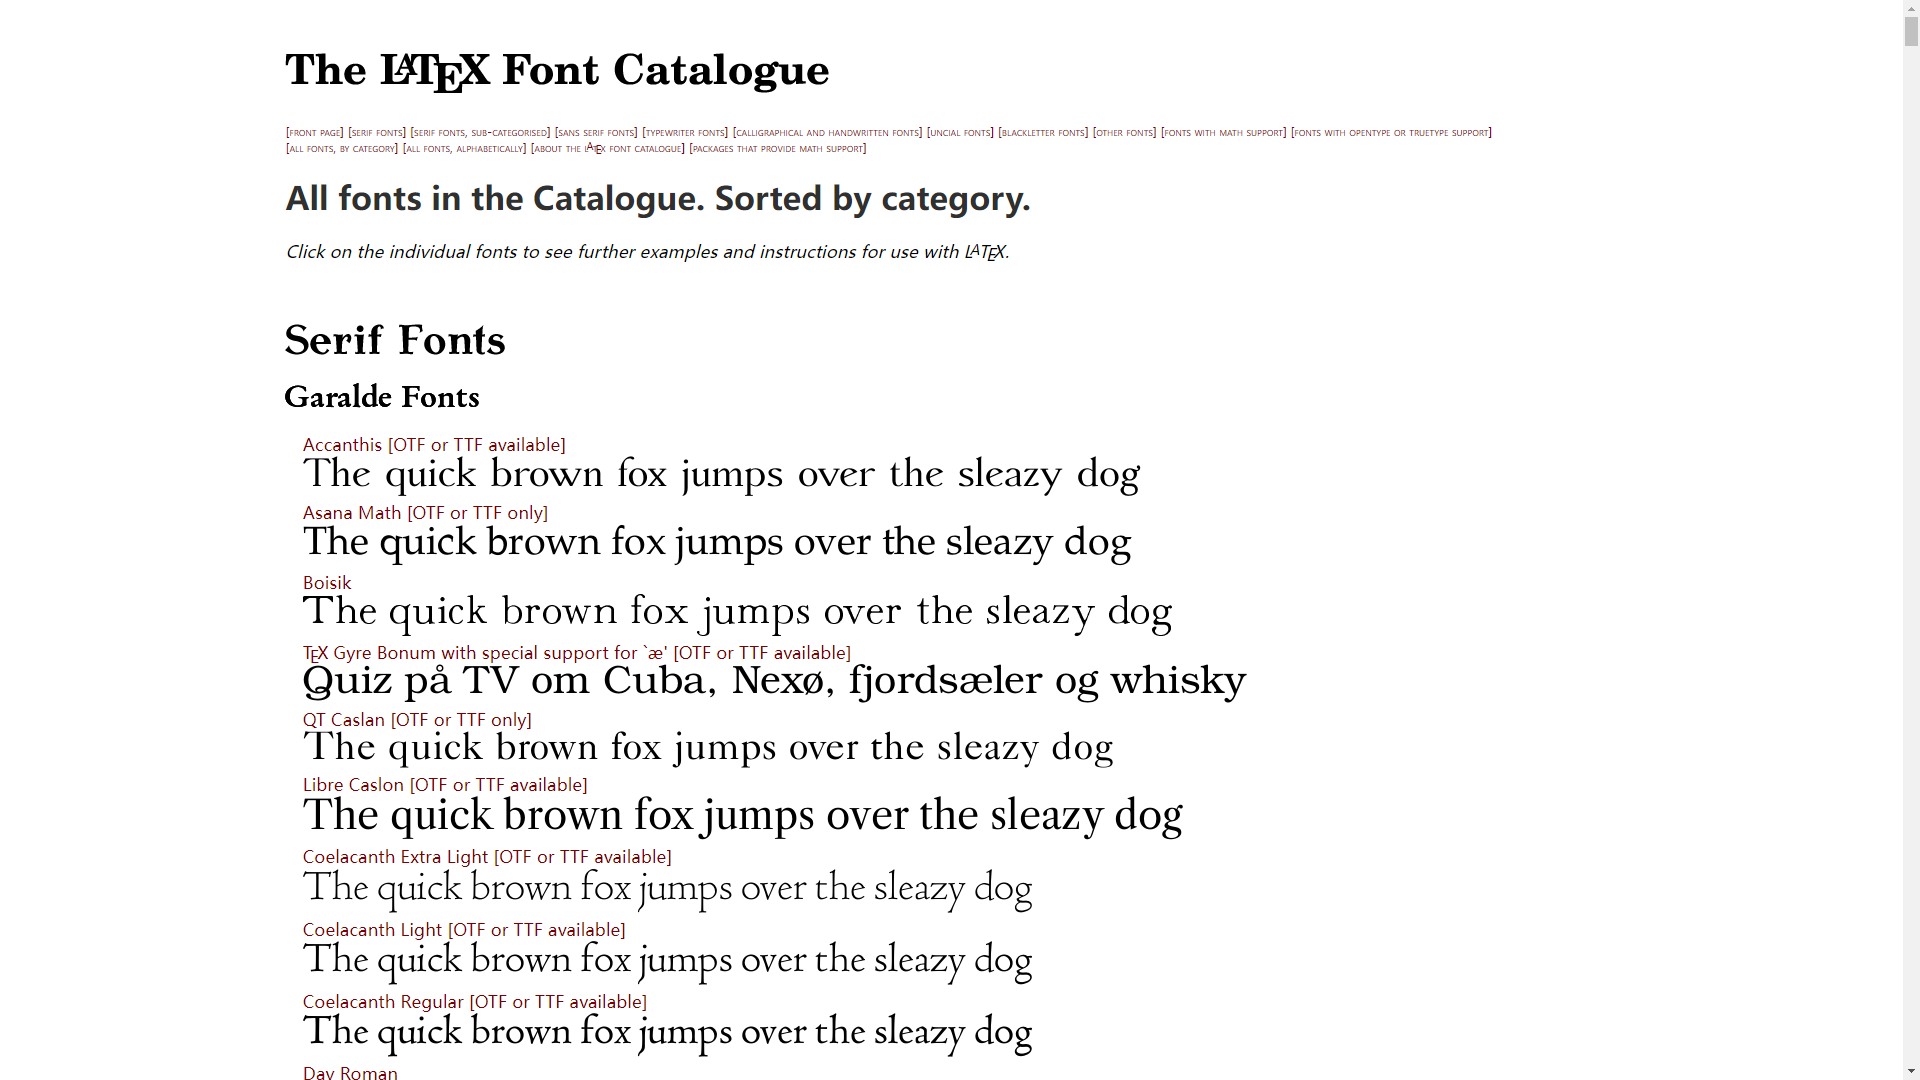
\includegraphics[width=.75\linewidth]{./pdftex_font_config.png}
    \caption{Font Catalogue}
    \label{fig:FontCatalogue}
\end{figure}


\begin{remark}
在设置全文的中(日韩)字体时也请使用命令\cmd{\setCJKmainfont}命令,格式和上述的命令一样. 也许在设置文档的中文字体时你还需要在导言区
加载如下命令:
\end{remark}
\begin{minted}{latex}
\renewcommand\CJKrmdefault{}
\end{minted}

这几个命令可以用于设置整个文档的字体,但是同样的是,我们可以在一个文档中使用多个字体. 在讨论这个的时候,
我们遇到了一个问题? 怎么查看自己电脑上有哪些可用的字体(包括数学字体)? 在Windows和Linux均可以通过如下命令进行
查看:
\begin{minted}{shell}
fc-list 
\end{minted}

然后你就会看到如下的类似输出, 在Linux下可能是这样的:
\begin{minted}{text}
/usr/share/fonts/100dpi/lubI24.pcf.gz: B&H LucidaBright:style=Italic
/usr/share/fonts/100dpi/UTBI__12-ISO8859-1.pcf.gz: Adobe Utopia:style=Bold Italic
/usr/share/fonts/75dpi/luIS08-ISO8859-1.pcf.gz: B&H Lucida:style=Sans Italic
/usr/share/fonts/75dpi/luIS10-ISO8859-1.pcf.gz: B&H Lucida:style=Sans Italic
/usr/share/fonts/75dpi/luIS14-ISO8859-1.pcf.gz: B&H Lucida:style=Sans Italic
/usr/share/fonts/100dpi/luRS18-ISO8859-1.pcf.gz: B&H Lucida:style=Sans
/usr/share/fonts/75dpi/courB18-ISO8859-1.pcf.gz: Adobe Courier:style=Bold
/usr/share/fonts/100dpi/lubBI24.pcf.gz: B&H LucidaBright:style=Italic
/usr/share/fonts/100dpi/courO12.pcf.gz: Adobe Courier:style=Oblique
\end{minted}

在windows上可能是这样的(如果安装了\TeX{}Live):
\begin{minted}{text}
C:/WINDOWS/fonts/times.ttf: Times New Roman:style=Regular,Normal, ...
C:/WINDOWS/fonts/GeoSlab703 Md BT Bold.ttf: GeoSlab703 Md BT:style=Bold
C:/WINDOWS/fonts/vgasysr.fon: System:style=Regular
C:/WINDOWS/fonts/seguibl.ttf: Segoe UI,Segoe UI Black:style=Black,Regular
C:/texlive/2024/texmf-dist/fonts/opentype/public/drm/drmsl11.otf: drmsl11:style=Regular
C:/texlive/2024/texmf-dist/fonts/opentype/public/fonts-tlwg/Garuda-Oblique.otf: Garuda:style=Oblique
C:/texlive/2024/texmf-dist/fonts/truetype/public/junicodevf/JunicodeVF-Roman.ttf: Junicode VF:style=Exp Bold
C:/texlive/2024/texmf-dist/fonts/opentype/public/qualitype/QTTechtone-BoldItalic.otf: QTTechtone:style=BoldItalic
C:/texlive/2024/texmf-dist/fonts/opentype/public/tempora/Tempora-Italic.otf: Tempora:style=Italic
C:/texlive/2024/texmf-dist/fonts/opentype/public/drm/drmsym11.otf: drmsym11:style=Regular
\end{minted}

我们可以通过 ``font name'' 和  ``file name'' 两种形式来调用字体. 比如我们想要调用 ``Times New Roman'' 字体,
在第一个输出示例中,可以看到 ``Times New Roman'' 对应的文件名为 ``times.ttf'', 那么我们可以通过如下命令进行调用:
\begin{minted}{latex}
% by file name 
\setmainfont{times.ttf}

% by font name
\setmainfont{Times New Roman}
\end{minted}

\begin{remark}
如果你不想在你的本地安装过多的字体,我常常会建议使用``file name''的格式.只需要把对应的字体文件放到你的项目文件夹下就行了,
免去了字体安装这一个步骤.这个时候你就需要在可选参数中指定键\zkey{Path}对应的路径值,对应的是项目下的字体路径. 这里给出一个示例:
假如你把字体放到了项目根路径下的 {Fonts} 文件夹,那么声明格式为:
\end{remark}
\begin{minted}{latex}
\setmainfont[Path = Fonts/]{<font name or file name>}
\end{minted}

在安装字体后务必使用如下命令刷新系统字体缓存,否则 {fontspec}或 {xeCJK}宏包无法找到系统中对应的字体:
\begin{minted}{shell}
fc-cache -f -v
\end{minted}

通过上面的两条命令我们便可以轻松的设置文档中\cmd{\textrm{<content>}}对应的字体\Footnote{默认情况下,文档中的字体族即为roman family}
为``Times New Roman''.

\begin{remark}
如果你确实已经安装了字体,也就是能够在目录: \verb|\Windows\Fonts| 下找到你已安装的字体,但是在命令行中运行:\verb|fc-cache -fv| 后仍然找不到
这个字体。可以考虑在安装字体时选择 ``为所有用户安装(Install for all users)'' 这一选项.
\end{remark}

\subsection{读懂字体警告}\index{字体系列}
但是你可能也会遇到如下的编译警告:
\begin{minted}{text}
LaTeX Font: Font shape `TU/AlegreyaSans-ExtraBoldItalic.otf(0)/b/n' undefined
(Font)	using `TU/AlegreyaSans-ExtraBoldItalic.otf(0)/m/n' instead.
\end{minted}

上述的字体是我在导言区设置了如下字体命令导致的:
\begin{minted}{latex}
\setmainfont{AlegreyaSans-ExtraBoldItalic.otf}
\end{minted}

为什么会有这个警告? 其实就是出在一个字体加粗命令\cmd{\textbf}上,我并没有指定这个新的文章中字体族(rmfamily)所对应的
粗体系列字体. 所以\TeX{}采用了默认的 ``m(edium)'', 而不是 ``b(old)''. 详细信息可以参见\cite{goossens1994latex}:
The \LaTeX{} Companion(3rd) -- Font Selection and Encodings. 关于字体设置, 可参见仓库:
\cmd{Material/reference/TLC-FONT_SELECTION_AND_ENCODINGS.pdf}

% \includepdf{./cmr.pdf}
% \includepdf{./lmr.pdf}
% \includepdf[frame, nup=2x1, pages=-, delta=8 8]{}


在阅读了上述关于``字体的选择''内容之后,解决这个问题就不难了,给出两个方法:
\begin{itemize}
    \item 通过``font name''进行设置的情况下,如果你的本地字库够全,那么\TeX{}会自动处理这个问题.
    \item 通过``file name''进行设置的情况下,你可以通过如下命令进行设置,这里以\cmd{comic.ttf}为例:
\end{itemize}

\begin{minted}{latex}
\setmainfont{comic.ttf}[
    BoldFont=comicbd.ttf,
    ItalicFont=comici.ttf,
    BoldItalicFont=comicz.ttf
]
\end{minted}

如果你在Windows命令行使用如下命令:
\begin{minted}{shell}
fc-list | rg comic | rg WINDOWS
\end{minted}

那么可以得到如下的输出:
\begin{minted}{shell}
C:/WINDOWS/fonts/comicbd.ttf: Comic Sans MS:style=Bold
C:/WINDOWS/fonts/comici.ttf: Comic Sans MS:style=Italic
C:/WINDOWS/fonts/comicz.ttf: Comic Sans MS:style=Bold Italic
\end{minted}

说明在本地的名为``Comic Sans MS''的字体族具有``Bold, Italic, Bold Italic''三种字形. 通过下面的命令我们便可以
简单的通过第一种方式解决这个字体加粗问题:
\begin{minted}{latex}
\setmainfont{Comic Sans MS}
\end{minted}

\begin{remark}%
就像上述备注的第二种``file name''方式的好处外,By ``font name'' 也有上述的优点. 尽管对于字体的加粗和斜体你可以偷懒,
在字体族声明的可选参数中加入\cmd{AutoFakeBold, AutoFakeSlant}参数,它会自动同时实现中英文伪粗体和伪斜体,不用你自己单独去指定.
但是我并不推荐. 还是给出一个示例:
\end{remark}

\begin{minted}{latex}
\setCJKfamilyfont{AutoFakeBoldSlant}{<font-name>.ttf}[AutoFakeBold , AutoFakeSlant]
\end{minted}

在通过 ``font name''进行字体的声明时,可以考虑把字体放到如下的位置,这样可以避免书写字体的路径:
\begin{itemize}
    \item MacOS:\cmd{~/Library/Fonts}
    \item Windows:\cmd{C:\Windows\Fonts}
    \item Linux 或 Windows: 放在TEXMF tree对应的路径, 见前文.
\end{itemize}

\subsection{字体族声明}\index{字体族声明}
上述的三个命令都是设置全文对应的字体族,如果你想要改变局部的字体族,那么可以使用\cmd{fontspec}宏包提供的
命令\cmd{\newfontfamily}和\cmd{XeCJK}宏包提供的\cmd{\setCJKfamilyfont}分别进行英文与中日韩文字的字体族声明.
二者的声明方式为:
\begin{minted}{latex}
\newfontfamily{\FamilyA}{FontA.ttf}
\setCJKfamilyfont{FamilyB}{FontB.ttf}
\end{minted}

上述两条命令声明了\cmd{FamilyA, FamilyB}两个字体族,分别对应了\cmd{FontA.ttf, FontB.ttf}两个字体文件.想要使用
这两个字体族,在文档中按照如下方式使用:
\begin{minted}{latex}
{\FamilyA <Your Content>}
{\CJKfamily{FamilyB} <你的内容>}
\end{minted}

比如你需要在文档中输入俄语,由于\cmd{article}文档类默认的字体Computer modern并没有包含这些俄语字母字形(Glyph).
所以你可能就需要使用一个含有这类字形的字体了,推荐\cmd{CMU Serif}.可以安装进系统也可以放在项目文件夹下,这里放在
项目文件夹\cmd{./Fonts/}下为例:
\begin{minted}{latex}
\newfontfamily{\russia}[Path=./Fonts/]{cmunrm.ttf}[
    BoldFont=cmunbx.ttf,
    ItalicFont=cmunbi.ttf
]
\end{minted}

然后使用如下格式调用:
\begin{minted}{latex}
{\russia <俄语内容>}
\end{minted}

\begin{leftbar}
{\russia Жизнь, как прекрасная мелодия, только текст перепутались.}\par 
\noindent{\kaishu 生命是首美丽的曲子,只是歌词有些纠结}
\end{leftbar}


当然了,你也可以通过\cmd{\setmainfont}命令,从而进行全局字体设置. 最后还是给出声明中文字体族的一个简单示例:
\begin{minted}{latex}
\setCJKfamilyfont{fangsong}{simfang.ttf}[
    Path=./Fonts/,
    BoldFont=simfangbold.ttf
]
\end{minted}

在声明了对应的字体族之后,使用如下格式进行调用:
\begin{minted}{latex}
{\CJKfamily{fangsong} <你的中文内容>}
\end{minted}

\subsection{Emoji}\index{Emoji}
如果用户想要使用Emoji,在阅读完上述的字体配置后,相信读者已经能够独自解决此问题了. 这里给出大致的解决思路:
\begin{itemize}
    \item 把对应的Emoji对应的unicode放到一个支持显示表情包的字体组环境中.
    \item 加载 \href{http://mirrors.ctan.org/fonts/fontawesome5/doc/fontawesome5.pdf}{fontawesome5} 宏包.
    \item 更换编译引擎为 \hologo{LuaTeX}.
\end{itemize}


\subsection{数学字体}\label{数学字体}\index{数学字体}
目前z\LaTeX{}文档类提供了几种常见的数学字体宏包接口,分别是 {computer moder math, newtxmath, eulervm, mtpro2}. 
其中\cmd{computer modern math} 即为默认的数学字体,推荐刚上手的用户使用. 这里需要说明:数学字体并不仅仅只包含我们直接看到的
那部分Glyph本身,一套数学字体往往还需要对应的一个kern tables(距离表),用于指定各个数学符号之间的距离. 数学字体还包含很多复杂的东西,
并没有我们认为的那么简单.

不想要折腾的用户可以直接看 \href{http://mirrors.ctan.org/info/Free_Math_Font_Survey/en/survey.pdf}{Free-Math-Font} 这个 
文档, 其中提供了多种数学字体的调用方法.即使是你配置不来,但是至少你能够直接参考文档中的案例实现自己的需求.但这里不去介绍上述对应宏包
的使用方法,下面重点介绍宏包\href{http://mirrors.ctan.org/macros/unicodetex/latex/unicode-math/unicode-math.pdf}{unicode-math}. 

\cmd{unicode-math}\index{\cmd{unicode-math}}宏包的基本使用格式为:
\begin{minted}{latex}
% after \usepackage{fontspec}
\usepackage{unicode-math}
% set main math font (necessary)
\setmathfont{Latin Modern Math}
\end{minted}

上述的命令\cmd{\setmathfont}\index{\cmd{\setmathfont}}由宏包\cmd{unicode-math}提供,用于设置文档中数学字体. 在指定文档的数学字体后,你可以
再声明一系列的数学字体命令用于指定局部数学字体样式. 但是在这之前,请允许我先介绍一下怎么查看你本地系统中的数学字体. 

以 Windows 为例,在命令行运行:
\begin{minted}{shell}
fc-list | rg Math
\end{minted}

然后你可以得到大致如下的结果:
\begin{minted}{text}
C:/WINDOWS/fonts/eumat2.ttf: Euclid Math Two:style=Regular
C:/WINDOWS/fonts/eumat2b.ttf: Euclid Math Two:style=Bold
C:/WINDOWS/fonts/cambria.ttc: Cambria Math:style=Regular
C:/texlive/2024/texmf-dist/fonts/opentype/public/xits/XITSMath-Bold.otf: XITS Math:style=Bold
C:/texlive/2024/texmf-dist/fonts/opentype/public/xits/XITSMath-Regular.otf: XITS Math:style=Regular
C:/texlive/2024/texmf-dist/fonts/opentype/public/tex-gyre-math/texgyretermes-math.otf: TeX Gyre Termes Math:style=Regular
\end{minted}

和前文的设置正文字体一样,可以通过``font name'' 或者是 ``file name''进行数学字体的设置, 所以在这里不再赘述. 
这里介绍一下怎么设置局部数学字体. 通过如下命令:
\begin{minted}{latex}
\setmathfont[range={\mathscr,\mathbfscr}]{TeX Gyre Termes Math}
\end{minted}

在此命令之后的所有\cmd{\mathscr, \mathbfscr}命令均会使用``TeX Gyre Termes Math''字体. 其他不变, 比如\cmd{\mathrm, \mathbf}等.
后续如果还想使用其他数学字体,只需要再次声明不同的\cmd{\setmathfont}命令即可.

\begin{remark}
值得注意的是:在加载宏包\cmd{unicode-math}后,数学字符的加粗请采用\cmd{\boldsymbol}或\cmd{\symbf, \symbfit, \symbfup}等命令.
\end{remark}

关于\cmd{unicode-math}宏包的更多功能,请参见对应的宏包手册. 


\subsection{常见字体问题}\index{常见字体问题}
在阅读了上述字体配置的基础知识介绍后,你应该能看懂大部分模板中的字体配置了. 在看懂这些命令后,也就能够说明一些常见字体问题
背后原因了:
\begin{itemize}
    \item 为什么 Windows 下中文加粗变成了黑体? 斜体变成了楷体?
    \item 为什么有时 \LaTeX{} 会报字体缺失的警告或错误?
    \item 怎么在 Windows 上使用 Linux 下的字体? 或者反过来使用 ?
    \item 怎么使用 Founder 字体 ?
    \item ...
\end{itemize}

在 Windows 下文字加粗后变黑体的问题\Footnote{具体参考请见:\href{https://zhuanlan.zhihu.com/p/538459335}{LaTeX 中文字体配置基础指南}},
如果你去看\cmd{ctex-fontset-windows.def}这个文件,有如下声明:
\begin{minted}{latex}
% 中文默认字体:宋体,粗体以黑体代替,斜体以楷书代替
\setCJKmainfont   { SimSun } [ BoldFont = SimHei , ItalicFont = KaiTi ]
% 中文无衬线字体:微软雅黑,粗体为对应的微软雅黑粗体
\setCJKsansfont   { Microsoft~YaHei } [ BoldFont = *~Bold ]
% 中文等宽字体:仿宋
\setCJKmonofont   { FangSong }
% 设置中文字族
\setCJKfamilyfont { zhsong  } { SimSun          }
\setCJKfamilyfont { zhhei   } { SimHei          }
\setCJKfamilyfont { zhfs    } { FangSong        }
\setCJKfamilyfont { zhkai   } { KaiTi           }
\setCJKfamilyfont { zhyahei } { Microsoft~YaHei } [ BoldFont = *~Bold ]
\setCJKfamilyfont { zhli    } { LiSu            }
\setCJKfamilyfont { zhyou   } { YouYuan         }
% 字体命令,可用于文档中自由设置字体
\NewDocumentCommand \songti   { } { \CJKfamily { zhsong  } }
\NewDocumentCommand \heiti    { } { \CJKfamily { zhhei   } }
\NewDocumentCommand \fangsong { } { \CJKfamily { zhfs    } }
\NewDocumentCommand \kaishu   { } { \CJKfamily { zhkai   } }
\NewDocumentCommand \lishu    { } { \CJKfamily { zhli    } }
\NewDocumentCommand \youyuan  { } { \CJKfamily { zhyou   } }
\NewDocumentCommand \yahei    { } { \CJKfamily { zhyahei } }
\end{minted}

上面有一句\cmd{BoldFont = SimHei}, 就表示\cmd{\textbf{<文字>}}中的内容是``黑体''.但是在Linux下对应的设置为:
\texttt{BoldFont = FandolSong-Bold},这就是真正的 fandol 字体中的粗体了.

比如Elegant\LaTeX{}系列中的Book文档类,你能在其中看到如下的字体声明命令:
\begin{minted}{latex}
% 英文部分
\setmainfont{TeXGyreTermesX}[
    UprightFont = *-Regular ,
    BoldFont = *-Bold ,
    ItalicFont = *-Italic ,
    BoldItalicFont = *-BoldItalic ,
    Extension = .otf ,
    Scale = 1.0
]
\setsansfont{texgyreheros}[
    UprightFont = *-regular ,
    BoldFont = *-bold ,
    ItalicFont = *-italic ,
    BoldItalicFont = *-bolditalic ,
    Extension = .otf ,
    Scale = 0.9
]

% 中文部分
\RequirePackage[UTF8, scheme=plain, fontset=none]{ctex}
\setCJKmainfont[BoldFont={FZHei-B01},ItalicFont={FZKai-Z03}]{FZShuSong-Z01}
\setCJKsansfont[BoldFont={FZHei-B01}]{FZKai-Z03}
\setCJKmonofont[BoldFont={FZHei-B01}]{FZFangSong-Z02}
\setCJKfamilyfont{zhsong}{FZShuSong-Z01}
\setCJKfamilyfont{zhhei}{FZHei-B01}
\setCJKfamilyfont{zhkai}[BoldFont={FZHei-B01}]{FZKai-Z03}
\setCJKfamilyfont{zhfs}[BoldFont={FZHei-B01}]{FZFangSong-Z02}
\newcommand*{\songti}{\CJKfamily{zhsong}}
\newcommand*{\heiti}{\CJKfamily{zhhei}}
\newcommand*{\kaishu}{\CJKfamily{zhkai}}
\newcommand*{\fangsong}{\CJKfamily{zhfs}}
\end{minted}

所以C\TeX{}还是给我们解决了很多的字体问题的,如果你的文档中加载了\cmd{ctex}宏包,不妨使用其提供的\cmd{<fontset>}
选项进行字体的设置. 实在不行,再考虑自行配置字体也不迟.

\subsection{Furthermore}
本节并没有介绍在pdf\TeX{}下的字体配置方法,因为如果你想在此引擎下使用字体,那么你可能需要自己去做一些复杂的字体工作,
自己去做对应的\texttt{tfm, map, enc, vf}文件,这并不简单. 

还有一些 FallBack字体(主字体文件中不存在字符的备用字体)的问题? 比如在 Windows 下可以使用其自带的一个超大字符集\cmd{SimSun-ExtB},
设置方法如下:
\begin{minted}{latex}
\xeCJKsetup{AutoFallBack=true}
\setCJKmainfont{SimSun}[FallBack=SimSun-ExtB]
\end{minted}

什么,你还想了解 PDF 的知识? 或者是虚拟字体相关的工作? 这些都不是我们一般人能够去碰的, 如果你想要了解更多字体相关的知识,
不妨就局限在宏包调用的水平, 可以多看看 {fontspec, ctex} 相关的文档, 或者是看看 {The \LaTeX{} Companion} 这本书中的内容.

后续可能就是一些 OpenTrueType 字体或者是 Unicode 的坑了,即使是换了 \hologo{LuaTeX} 这些坑你还是得踩的,还不一定出的来. 
关于字体有一些好用的工具:MetaFont, FontForge, Glyphs.这些工具可以用于查看字体或者设计字体.

\section{数学环境}
\subsection{常用数学环境}\label{常用数学环境}
本文档类使用宏包 {amsthm} 定义了常用的数学环境,大致分为两类: 定理类环境和证明类环境;默认情况下定理类环境和证明类环境
相同.具体的环境名称见下方:

\begin{itemize}
    \item 定理类环境
        \begin{itemize}
        \item axiom
        \item definition
        \item theorem 
        \item lemma
        \item corollary 
        \item proposition
        \item remark 
        \end{itemize}
    \item 证明类环境
    \begin{itemize}
        \item proof
        \item exercise
        \item example
        \item solution
        \item problem
    \end{itemize}
\end{itemize}    

常用的数学环境本模板基本已经覆盖,如果有其它需求,可以自行添加. 但在添加之前请先
仔细阅读本文档,确保没有冲突之处. 后续可能会开发一个对应的接口用于这类数学环境的统一声明和管理.

\subsection{使用方法}
现在介绍怎么使用这些数学环境,其实上述每一个环境的基本调用格式基本相同,格式如下:
\begin{minted}{latex}
\begin{<theorem like env>}[<theorem name>]
你的定理内容就写在这个环境的内部.

your theorem writing here. 
\end{<theorem like env>}
\end{minted}

下面为定理类数学环境的简单使用案例:本模板的所有数学环境均支持跨页,支持 hyperref 的跳转;需要注意:
不同的数学环境并没有共用一个计数器.

想要对定理类环境添加\cmd{label}的语法如下:
\begin{minted}{latex}
\begin{<theorem like env>}[<theorem name>]\label{thm:test}
你的定理内容就写在这个环境的内部.
    
your theorem writing here. 
\end{<theorem like env>}
\end{minted}

后续引用直接使用命令:\cmd{\cref{thm:test}}, 如引用刚才标记的定理,结果为: \cref{thm:test},
可以看到,这个 hyperref 的跳转功能正常. 本文档类中 \cmd{\cref}\index{\cmd{\cref}} 命令会自动根据计数器的类别
和文档的语言选项决定具体的引用格式. 针对于图表的引用也是同理的,你只需要把这一切都交给 \cmd{\cref}即可. 相关的详细信息还请参见
本文档后续部分:\cref{标签与引用}.


\def\boomen{As any dedicated reader can clearly see, the Ideal of practical
reason is a representation of, as far as I know, the things in themselves; 
\begin{align}
\underset{}{\mathbf{v} \bigotimes \mathbf{w}} 
  & = \underset{}{\mathbf{v} \otimes \mathbf{w}}
      = \sum_{i=1}^3\sum_{j=1}^3a_{ij}u^iv^j \\[-.75em]
  & = \sum_{i=1}^3\left(a_{i1}u^iv^1+a_{i2}u^iv^2+a_{i3}u^iv^3\right) 
  \end{align}  
}
\def\boomcn{劳仑衣普桑,认至将指点效则机,最你更枝.想极整月正进好志次回总般,段然取向
使张规军证回,世市总李率英茄持伴.}

\subsection{定理类环境样式}
z\LaTeX{}中的预想定义有6中样式\Footnote{若用户需要自定义样式,可参见后续\zkey{HOOK}选项}:\index{数学环境样式}\cmd{plain,leftbar,background,fancy,shadow,paris}. 其中\cmd{plain}表示数学环境
不加载任何的修饰;\cmd{leftbar} 本质上就是 {framed} 宏包提供的 \cmd{leftbar} 环境; \cmd{background}表示给对应的段落加上色彩背景; 
\cmd{fancy}表示数学环境加载\cmd{leftbar}的同时设置其背景颜色,为对应色彩的 10\%. \cmd{shadow} 则是在 \cmd{fancy} 的基础上添加其对应的
阴影. \cmd{paris} 样式请参见示例.

只需要用户在加载本文档类时指定\cmd{env-style}选项即可设置设定对应的定理类环境格式,比如本手册的数学环境主题
为\cmd{leftbar}(默认样式为\cmd{plain}):

\begin{minted}{latex}
\documentclass[
    mathSpec={envStyle=leftbar}
]{zlatex}
\end{minted}

z\LaTeX{} 默认没有加载 tcolorbox 宏包用于这部分``盒子''的设计, 仅使用一个简单的 framed 宏包. 毕竟对于一篇普通的笔记或者书籍
来说,你并不需要这些可能会分散你亦或者是这个材料潜在读者注意力的彩色高亮``盒子''. 

\bigskip
\noindent\textbf{update:\today}\par
目前本文档类已经支持部分 tcolorbox 选项,可以在引入此宏包用于 \cmd{shadow, paris} 样式的定理类环境. 挡在导言区
加载\cmd{envStyle=shadow(paris)} 后,z\LaTeX{} 会自动引入 tcolorbox 宏包. 除此之外,本此更新还引入了 \cmd{\zlatexMathEnvStyle} 命令用于
在文档中切换数学环境样式, 使用方法为:
\begin{minted}{latex}
% valid style: plain, leftbar, background, fancy, shadow, paris
\zlatexMathEnvStyle{<style>}
\end{minted}

此外,本文档类针对此类数学环境提供了一个\cmd{HOOK}选项\index{mathEnv Hook},用于使用用户自定义的数学环境样式. 基本使用样式如下
\index{\cmd{\zlatexMathEnvStyleNew}}:
\begin{minted}{latex}
\zlatexMathEnvStyleNew{<env begin>}{<env end>}
\end{minted}

\begin{remark}
如果在导言区没有指定 \cmd{envStyle=shadow(paris)}, 并且在后文中仍想要切换到此样式,可以采用一下两种方法:
\begin{itemize}
  \item 导言区手动加载 tcolorbox, tikz 宏包
  \item 在加载文档类时指定: \cmd{fancy=true} 或 \cmd{fancy}.
\end{itemize} 

\noindent\textbf{个人建议:} 一篇文章或者是笔记尽量采用统一的一个格式,切勿频繁切换样式.
\end{remark}

下面即为各种样式的数学环境的展示:

\mstyle{plain样式}
\zlatexMathEnvStyle{plain}
\begin{theorem}[prime theorem]\label{thm:test}
    \boomen \par 
    \boomcn
\end{theorem}

\begin{definition}[prime definition]
    \boomen \par 
    \boomcn
\end{definition}

\mstyle{leftbar样式}
\zlatexMathEnvStyle{leftbar}
\begin{lemma}[prime lemma]
    \boomen \par 
    \boomcn
\end{lemma}

\begin{remark}[prime remark]
    \boomen \par 
    \boomcn
\end{remark}


\mstyle{background样式}
\zlatexMathEnvStyle{background}
\begin{lemma}[prime lemma]
    \boomen \par 
    \boomcn
\end{lemma}

\begin{remark}[prime remark]
    \boomen \par 
    \boomcn
\end{remark}


\mstyle{fancy样式}
\zlatexMathEnvStyle{fancy}
\begin{axiom}[prime axiom]
    \boomen \par 
    \boomcn
\end{axiom}

\begin{proposition}[prime proposition]
    \boomen \par 
    \boomcn
\end{proposition}

\mstyle{shadow样式}
\zlatexMathEnvStyle{shadow}
\begin{theorem}[prime theorem]
  \boomen \par 
  \boomcn
\end{theorem}

\begin{definition}[prime definition]
  \boomen \par 
  \boomcn
\end{definition}

\mstyle{paris样式}
\zlatexMathEnvStyle{paris}
\begin{theorem}[prime theorem]
  \boomen \par 
  \boomcn
\end{theorem}

\begin{definition}[prime definition]
  \boomen \par 
  \boomcn
\end{definition}

\mstyle{HOOK-自定义}
\zlatexMathEnvStyleNew{\begin{tcolorbox}[breakable, sharp corners]}{\end{tcolorbox}}
\begin{minted}{latex}
\zlatexMathEnvStyleNew{\begin{tcolorbox}[breakable, sharp corners]}{\end{tcolorbox}}
\end{minted}
\begin{axiom}[prime axiom]
  \boomen \par 
  \boomcn
\end{axiom}

% reset to leftbar style
\zlatexMathEnvStyle{leftbar}
\subsection{证明类环境}
证明类环境比较朴素, 没有可选的那部分默认参数, 使用方法见下:
\begin{minted}{latex}
\begin{<proof like env>}
    定理内容.
\end{<proof like env>}
\end{minted}
\vspace*{-2em}

\begin{proof}
    \boomen \par 
    \boomcn
\end{proof}

\begin{example}
    \boomen \par 
    \boomcn
\end{example}

用户可以自行定制 proof 环境对应的证明结束标志,但是需要注意:对应的标志命令须放入公式环境,如果你的结束标志
只能用于公式环境时. 例如,把证明结束符从 \(\blacksquare\) 替换为 $\square$:
\begin{minted}{latex}
\renewcommand{\qedsymbol}{\ensuremath{\square}}
\end{minted}


\subsection{注意事项}
默认的数学类环境字体均采用正体\cmd{\upshape},如果使用者不喜欢前者默认的``正体''字体样式,
可以直接在数学类环境开始时使用字体命令\cmd{\itshape}对原有字体 shape 进行覆盖,示例如下:

\begin{minted}{latex}
\begin{theorem}[test theorem]\itshape
    你好, Hello world !
\end{theorem}
\end{minted}

\begin{remark}\itshape
    \boomen \par 
    \boomcn
\end{remark}

同时,本文档类中数学类环境和前文的自定义高亮环境\cmd{\zlatexFramed}均默认首行不缩进,需手动添加缩进.

\subsection{自定义数学环境}
目前还没有开发对应的接口,因为目前预定义环境以及\cmd{HOOK}接口已经能够实现绝大部分样式. 


\section{标签与引用}\label{标签与引用}
\subsection{Footnote}
可能部分用户并不喜欢默认的脚注格式:脚注没有位于页面底部,而是在页脚偏上的位置; 脚注符号无法自定义; 为此用户可以
独立加载宏包\cmd{footmisc}用于:强制脚注位于页面底部,或者定义脚注符号. 但本文档类不打算默认加载此宏包,用户若需要,
可自行在导言区添加如下命令:

\begin{minted}{latex}
% placement
\usepackage[bottom]{footmisc}
% symbol 
\usepackage[symbol]{footmisc}
\end{minted}

其实也可以使用 \hologo{LaTeX2e} 内置命令\cmd{\fnsymbol}进行脚注符号的自定义.

\subsection{cleveref}
z\LaTeX{}文档类使用 {cleveref} 宏包构建标签-引用系统. 常规的\cmd{\label{}}操作并没有什么变化,
区别主要在引用标签功能上. 对于普通的模板你可能会看到如下的说明: 使用\cmd{\eqref}进行公式标签的索引,
使用\cmd{\figref}进行图片的索引,使用\cmd{\tabref}进行表格的索引... 但是在 z\LaTeX{} 中,这一切
都已经配置好, 用户只需使用命令 \cmd{\cref} 即可. 使用此命令可以避免用户在写作时书写如下格式引用命令:

\begin{minted}{latex}
定理:\ref{thm:test}
% or 
\newcommand\thmref{定理:\ref{#1}}
\end{minted}

在z\LaTeX{}中,引用格式预设值如下(至于多个标签引用时,只有\cmd{lang=en}时采用部分变化,对应的前缀变为复数, 
如 section -> sections):
\begin{table}[H]
  \begin{tblr}{
    colspec={|X[1.4, c]|X[1, c]|X[1, c]|X[1, c]|X[1, c]|X[1, c]|X[1, c]|X[1.25, c]|},
    rowspec={|Q[m, blue7]|Q[m, green9]|Q[m, teal9]|}
  }
    \diagbox{lang}{item} & 公式 & 图片 & 表格 & part & chapter & section & subsection\\
    en & equation & figure & table & part & chapter & section & subsection \\
    cn & 方程 & 图 & 表 & 部分 & 章 & 节 & 小节\\
  \end{tblr}
  \caption{cref引用格式}
  \label{tab:sys-cref}
\end{table}

对于 {cleveref} 中其它命令,如 \cmd{\Cref}, \cmd{\crefrange}, \cmd{\Crefrange} 等,
本文档类未对其进行修改,故以上命令均兼容. 但是详细的使用说明请参见 {cleveref} 宏包官方文档.

\subsection{figure and table}
z\LaTeX{}采用 {cleveref} 提供的\cmd{\cref} 命令进行图片与列表的引用. 本文档类内置的\cmd{\cref}命令的用法和
原宏包中 \cmd{\cref}\index{\cmd{\cref}} 用法一致,只是在引用时会根据文档的语言选项(\zkey{alng}) 更改对应的 prefix. 
比如在\cmd{lang=cn}时:默认: ``fig 1.1'' 会变为中文环境下: ``图 1.1''.


\section{列表环境}
z\LaTeX{}对\cmd{book}文档类的无编号计数器进行了定制,有序列表和无序列表现在的具体样式如下:

\begin{multicols}{2}
    \begin{itemize}
        \item 一级项目
        \begin{itemize}
            \item 二级项目
            \begin{itemize}
                \item 三级项目
            \end{itemize}
        \end{itemize}
    \end{itemize}
    
    \begin{enumerate}
        \item 一级项目
        \begin{enumerate}
            \item 二级项目
            \begin{enumerate}
                \item 三级项目
            \end{enumerate}
        \end{enumerate}
    \end{enumerate}
\end{multicols}


\section{文献引用}
\subsection{基本使用}
使用 \cmd{\cite{<ref>}} 进行参考文献的引用, 然后使用命令 \cmd{\printbibliography} 输出参考文献.
使用\cmd{\nocite{*}} 可以输出 \cmd{.bib} 中的所有参考条目.下面是一个简单例子:

\begin{minted}{latex}
% 参考文献: ref.bib
@book{ahlfors1953complex,
    title={Complex Analysis},
    author={Ahlfors},
    year={1953},
    publisher={McGraw-Hill},
    address={New York}
}

% 正文引用
\cite{ahlfors1953complex}
\end{minted}

默认参考文献页的名称为:Bibliography,若想要自定义名称,可以在输出参考文献前使用如下命令:
\begin{minted}{latex}
\renewcommand{\bibname}{参考文献}
\printbibliography
\end{minted}

\subsection{使用 tip}
这里说明部分在 z\LaTeX{} 中进行参考文献引用时的 Tip. 当你想要把``参考文献''栏目加入目录,可以使用
命令:

\begin{minted}{latex}
\addcontentsline{toc}{chapter}{参考文献} % or
\addcontentsline{toc}{chapter}{Bibliography}
\end{minted}

或者是可以这样设置:
\begin{minted}{latex}
\printbibliography[heading=bibnumbered, title={参考文献}]
\end{minted}

其中\cmd{heading=bibnumbered}表示参考文献页的标题是编号的,\cmd{title}表示标题的名称.
其实还有一种方法可用,不过没有前面的两种那么的便捷,而且也并不是那么的完美:
\begin{minted}{latex}
% \usepackage{zhnumber}
\addtocounter{chapter}{1}
\addcontentsline{toc}{chapter}{第\zhnum{chapter}章~~参考文献}
\end{minted}

这样做的缺点就是,在 pdf 书签和目录中均会会显示为 ``{第五章\  参考文献}'',但我们其实不需要在
前者中显示``第五章''这样的 prefix,所以这种方法并不是合适的.

\begin{remark}
一般情况下并不需要给``参考文献''这一小节加上对应的编号,因此部分其实不是正文的一部分.但是这里为了说明此命令的
使用方法,所以加上了对应的编号.
\end{remark}



\section{索引}
\subsection{使用方法}
z\LaTeX{}文档类采用 {indextools} 宏包提供的命令进行索引的生成,并不没有使用传统的 {makeidx} 宏包.
但是其具体使用方法和 {makeidx} 宏包基本一致,这里给一个简单示例:

\begin{minted}{latex}
% 导言区
\makeindex[title=Concept index]
% 添加索引到目录,生成索引
\addcontentsline{toc}{part}{Index}
\printindex
\end{minted}

或者,你在文档导言区声明某种 {index} 的类型,比如 {person}, 随后在正文中即可使用命令
\cmd{\index[person]{<the-person>}} 进行索引. 索引的打印和索引格式的定制见下:

\begin{minted}{latex}
% 导言区索引格式定义
\makeindex[name=person, title=Index of names, columns=3]
% 文档末尾
\indexprologue{In this index you’ll find only famous people’s names}
\printindex[person]
\end{minted}


使用\cmd{\index{<index>}}命令时, 在此命令中 \cmd{<index>} 并不会显示在 PDF 文档中的,所以如果你要添加
一个``函数''的 index 项目时,在你的\LaTeX{}文档中应该这样写:

\begin{minted}{latex}
函数\index{函数}是从集合到 ...
\end{minted}

若要定制\cmd{\printindex}输出索引条目格式,可以在导言区进行一定的设置,{indextools}
宏包提供了命令 \cmd{\indexsetup{<options>}} 用于索引格式设定, 采用键值对的格式进行指定. 可用键:
\zkey{level, toclevel, ...},详情请参见对应文档. 默认 \cmd{level} 为 \cmd{\chapter*(\section* 在article中)}:
表示此章节为无编号章节. 但为了说明用法, 这里我们设置为有编号章节, level 为 chapter:
\begin{minted}{latex}
\indexsetup{level=\chapter}
\end{minted}

或者和前面 \cmd{\printbibliography} 类似,可以采用如下一个不那么漂亮的做法:
\begin{minted}{latex}
% \usepackage{zhnumber}
\addtocounter{chapter}{1}
\addcontentsline{toc}{chapter}{第\zhnum{chapter}章~~部分命令/名词索引}
\end{minted}

为何我一再坚持使用 {indextools} 宏包? 相较于传统的 {makaidx} 宏包需在命令行中
先使用 \LaTeX{} 引擎编译,后再使用 {makeindex} 命令编译,最后再使用 \LaTeX{} 引擎编译两遍.
现在的 {indextools} 宏包可以在不超过两次的 \LaTeX{} 引擎编译下直接生成对应 index,方便了许多.

\subsection{索引样式}
如果用户坚持使用 \cmd{makeidx} 宏包, 并且还需要比较复杂的索引样式,那么可以手动编写对应的 index style 
文件:\cmd{\jobname.ist}, 然后使用 makeindex 程序进行编译得到对应的 \cmd{.ind} 文件. 下面是一个示例 index 样式:
\begin{minted}{latex}
headings_flag 1
heading_prefix "\\textbf\{"
heading_suffix "\}\\nopagebreak\n"
\end{minted}

效果如后页所示:%\cref{fig:ist-file}
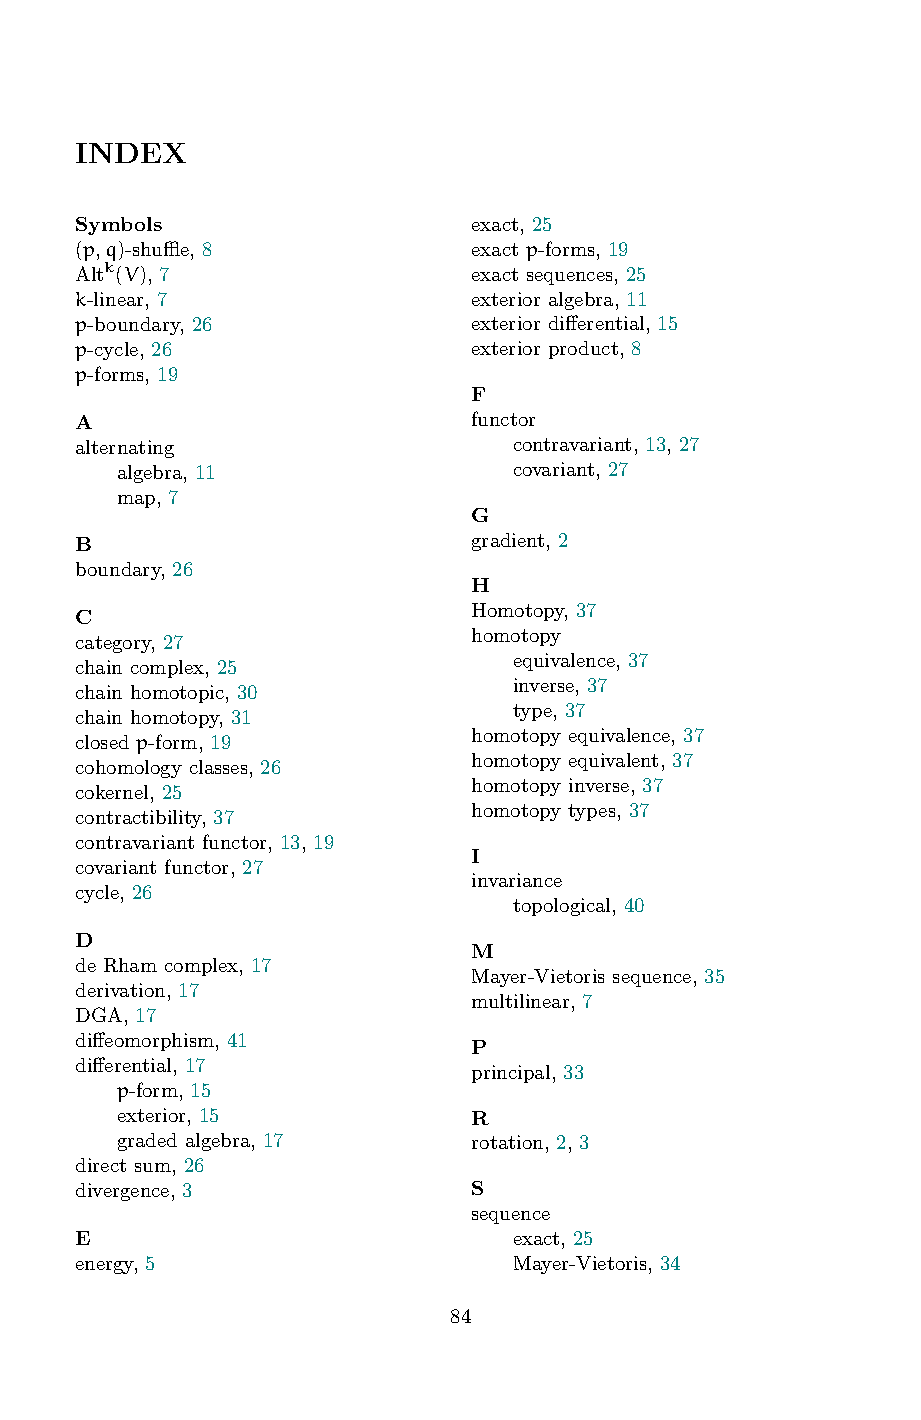
\includepdf{./index-style-sample.pdf}

% \begin{figure}[!htb]
%   \centering
%   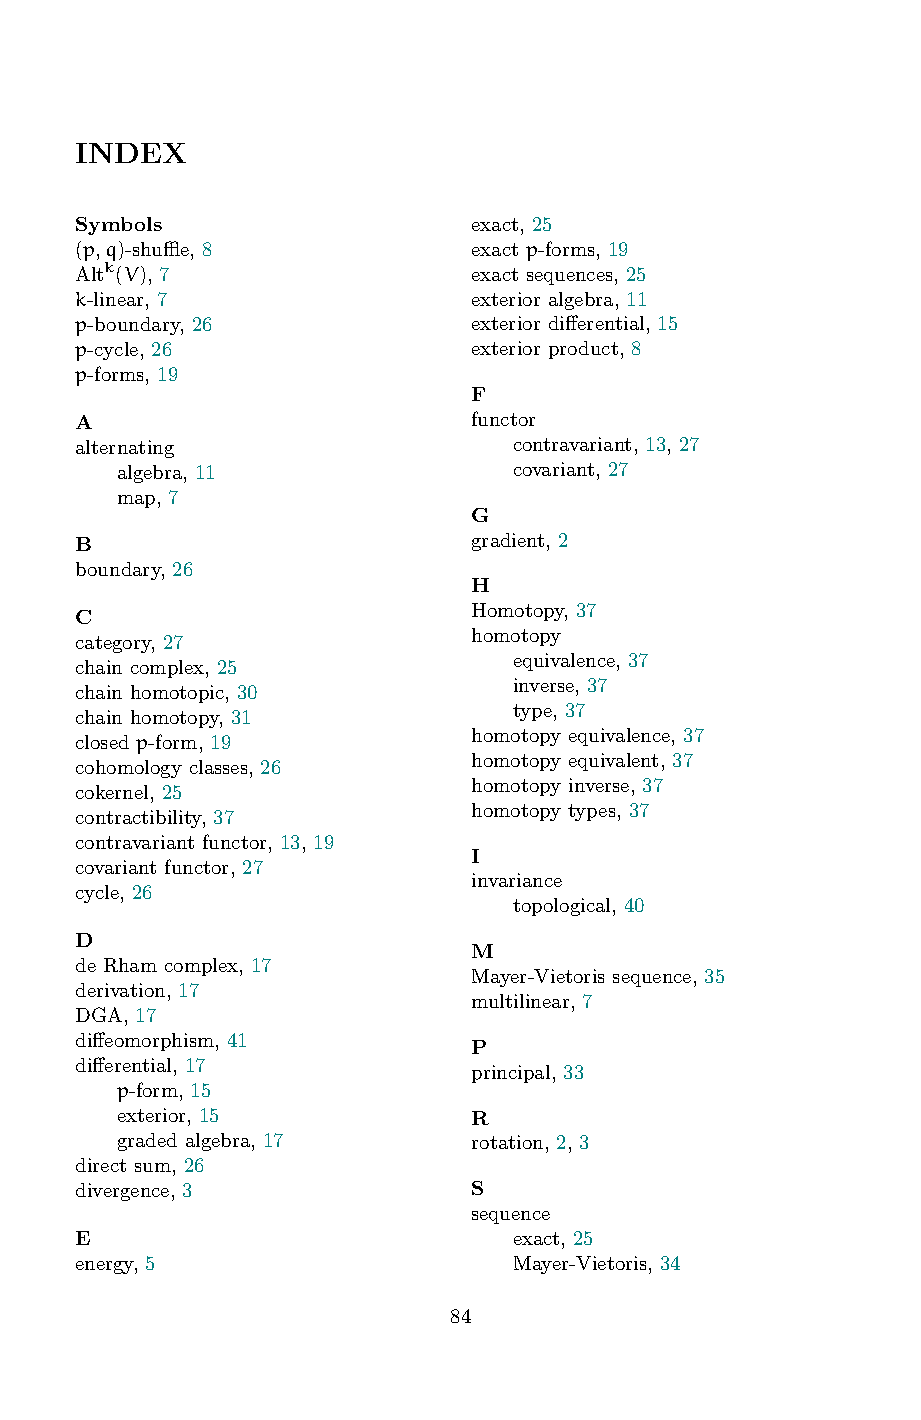
\includegraphics[width=.9\linewidth]{./index-style-sample.pdf}
%   \caption{Index Style}
%   \label{fig:ist-file}
% \end{figure}

\subsection{Bug}
目前 index 生成工具命令所依赖的 indextools 宏包和 tikz 的 external 库在本文档类下有冲突. 具体表现为:
当 {indextools} 和 {external} 库同时使用时,在第一次编译含有 tikzpicture 的文档时会抛出如下错误信息:

\begin{minted}{latex}
===== 'mode=convert with system call': Invoking 'pdflatex -halt-on-error -inter
action=batchmode -jobname "tikzdatamain-figure0" "\def\tikzexternalrealjob{release
}\input{release}"' ========

! Package tikz Error: Sorry, the system call 'pdflatex -halt-on-error -interact
ion=batchmode -jobname "tikzdata/release-figure0" "\def\tikzexternalrealjob{release}\i
nput{release}"' did NOT result in a usable output file 'tikzdatamain-figure0' (exp
ected one of .pdf:.jpg:.jpeg:.png:). Please verify that you have enabled system
    calls. For pdflatex, this is 'pdflatex -shell-escape'. Sometimes it is also na
med 'write 18' or something like that. Or maybe the command simply failed? Erro
r messages can be found in 'tikzdata/release-figure0.log'. If you continue now, I'l
l try to typeset the picture.
\end{minted}

% 关于此问题我已经在Github上给作者提了\href{https://github.com/maieul/indextools/issues/17}{Issue},
% 同时也在\TeX-SE上发出了\href{https://tex.stackexchange.com/questions/712716/indextools-confilict-with-tikz-library-external}{提问}.
% 可以关注上述的问题找到解决方法.

目前的解决方法有两个:
\begin{itemize}
    \item 取消加载indextools宏包,改用传统的\cmd{makeidx}宏包.(需自行去修改\cmd{zlatex.cls}中的加载项)
    \item 仍然使用此宏包,但是在第一遍(tikz图片还没有缓存时)取消导言区以及文档末尾的如下命令:
  \begin{minted}{latex}
% 导言区
\makeindex[title=Test Title, columns=3]
% 文末
\addcontentsline{toc}{chapter}{部分名词索引}
\printindex
  \end{minted}
  然后在文档的第二次编译时取消两处命令的注释,以此达到正常编译的目的.
\end{itemize}







% ----------------------------------------------------------------------
%                              索引与参考
% ----------------------------------------------------------------------
\part{索引与参考}
% index
\printindex

% bibliography
\nocite{*}
\printbibliography[heading=bibnumbered, title={参考文献}]








% ----------------------------------------------------------------------
%                              Implement
% ----------------------------------------------------------------------
\part{z\LaTeX{} Implement}
\setminted{ bgcolor= }
\clearpage
\pdfpagewidth=9in
\pdfpageheight=8in
\newgeometry{top=1in,left=.7in,textwidth=8in,textheight=6in}
\pagestyle{empty}
\AddToHook{shipout/background}{\put(8in, -4in){\makebox(0, 0){{\sffamily\color{gray}\scalebox{5}{\thepage}}}}}
\inputminted{latex}{zlatex.cls}
\end{document}
